\documentclass[main]{subfiles}

\begin{document}
% Chapter Template
\setcounter{chapter}{1}

% Evolutionary Optimization
% Basic components
%  Universe, Planets and Environments
%   Planet Physics
%  Epochs
%   Fitness functions
%  Populations
%  Creatures
%   Genotypes
%   Phenotypes
%    Constrained Rigid body model
%    Featherstone Multi-rigidbody model
%  Model organisms
% Reaper
%  Crossover
%  Mutations
% Evaluation Step
% Variation Step
\chapter{Evolutionary Optimization} % Main chapter title

\label{Chapter\thechapter} % Change X to a consecutive number; for referencing this chapter elsewhere, use \ref{ChapterX}

\lhead{Chapter \thechapter. \emph{Evolutionary Optimization}} % Change X to a consecutive number; this is for the header on each page - perhaps a shortened title

The following chapter describes the evolutionary optimization algorithm as it is implemented in the Minemonics simulator. %
%
The Minemonics simulator is the experimentation platform used throughout this thesis and is a project that was developed from scratch, mainly because other simulators for evolving virtual creatures are unpublished by the respective research groups, are outdated, or implement a different type of simulation than is needed to simulate the model described in this thesis. %
%
Apart from the research interests, the simulator was made to be extensible for other research experiments to be implemented. %
%
It is available open-source from its git repository on Github \cite{bib:Minemonics2016}.

\section{Basic Components}
% rev. 2

To understand the purpose of the simulation, it is important to first understand its different components. %
%
Therefore, the basic components of the simulator and their respective features are discussed first. %
%
Components are described from coarse to fine grain, starting with the universe and ending with the genomic and phenomic structure of a simulated individual.

\begin{figure}[H]
\hspace*{-1.2in}
\begin{tikzpicture}
\pgfdeclarelayer{background}
\pgfdeclarelayer{foreground}
\pgfsetlayers{background,main,foreground}
\tikzstyle{bigbox} = [draw=black!80, thick, fill=black!5, rounded corners, rectangle]
\tikzstyle{box} = [minimum size=0.6cm,draw=black!80, thick,rounded corners, rectangle, fill=black!20]

%###############################################
% Universe and anchors
%###############################################
\node[align=center,box](universe-node){
Universe
};
\node(universe-left-zoom-node)[below left=-0.1cm and -0.3cm of universe-node]{};
\node(universe-right-zoom-node)[below right=-0.1cm and -0.3cm of universe-node]{};


%###############################################
% Planets and anchors
%###############################################
\matrix[anchor=east](planets)[below=1cm of universe-node, row sep=2mm, column sep=2mm, inner sep=2mm] {
\node(left-planet-node)[box]{Planet}; & \node[box]{}; & \node[box]{}; & \node[]{$\dots$}; & \node(planet-node)[box]{Planet}; & \node[]{$\dots$}; & \node[box]{}; & \node[box]{}; & \node(right-planet-node)[box]{Planet};\\
};
\node(planet-left-row-node)[above left=-0.1cm and -0.3cm of left-planet-node]{};
\node(planet-right-row-node)[above right=-0.1cm and -0.3cm of right-planet-node]{};

%###############################################
% Lines between universe and planets
%###############################################
\draw (universe-left-zoom-node) -- (planet-left-row-node);
\draw (universe-right-zoom-node) -- (planet-right-row-node);

\fill [path fading=south,black!10] (universe-left-zoom-node.center) to (universe-right-zoom-node.center) to (planet-right-row-node.center) to (planet-left-row-node.center) to (universe-left-zoom-node.center);

%###############################################
% Planet anchors
%###############################################
\node(planet-left-zoom-node)[below left=-0.1cm and -0.3cm of planet-node]{};
\node(planet-right-zoom-node)[below right=-0.1cm and -0.3cm of planet-node]{};


%###############################################
% Planet components and anchors
%###############################################
\matrix[anchor=east](planet-components)[below=1cm of planet-node, row sep=2mm, column sep=2mm, inner sep=2mm] {
\node(environment-node)[box]{Environment}; & \node(evolutionary-process-node)[box]{Evolution};\\
};
\node(planet-components-left-row-node)[above left=-0.1cm and -0.3cm of environment-node]{};
\node(planet-components-right-row-node)[above right=-0.1cm and -0.3cm of evolutionary-process-node]{};

%###############################################
% Lines between planet and planet components
%###############################################
\draw (planet-left-zoom-node) -- (planet-components-left-row-node);
\draw (planet-right-zoom-node) -- (planet-components-right-row-node);

\fill [path fading=south,black!10] (planet-left-zoom-node.center) to (planet-right-zoom-node.center) to (planet-components-right-row-node.center) to (planet-components-left-row-node.center) to (planet-left-zoom-node.center);

%###############################################
% Evolutionary Process anchors
%###############################################
\node(evolutionary-process-left-zoom-node)[below left=-0.1cm and -0.3cm of evolutionary-process-node]{};
\node(evolutionary-process-right-zoom-node)[below right=-0.1cm and -0.3cm of evolutionary-process-node]{};

%###############################################
% Evolutionary Process Components and Anchors
%###############################################
\matrix[anchor=east](evolutionary-process-components)[below left=1cm and -2cm of evolutionary-process-node, row sep=2mm, column sep=2mm, inner sep=2mm] {
\node(reaper-node)[box]{Reaper}; & \node(populations-node)[box]{Populations};\\
};
\node(evolutionary-process-components-left-row-node)[above left=-0.1cm and -0.3cm of reaper-node]{};
\node(evolutionary-process-components-right-row-node)[above right=-0.1cm and -0.3cm of populations-node]{};

%###############################################
% Lines between evolutionary process and evolutionary process components
%###############################################
\draw (evolutionary-process-left-zoom-node) -- (evolutionary-process-components-left-row-node);
\draw (evolutionary-process-right-zoom-node) -- (evolutionary-process-components-right-row-node);

\fill [path fading=south,black!10] (evolutionary-process-left-zoom-node.center) to (evolutionary-process-right-zoom-node.center) to (evolutionary-process-components-right-row-node.center) to (evolutionary-process-components-left-row-node.center) to (evolutionary-process-left-zoom-node.center);

%###############################################
% Evolutionary Process components anchors
%###############################################
\node(populations-left-zoom-node)[below left=-0.1cm and -0.3cm of populations-node]{};
\node(populations-right-zoom-node)[below right=-0.1cm and -0.3cm of populations-node]{};

%###############################################
% Populations and anchors
%###############################################
\matrix[anchor=east](populations)[below=1cm of populations-node, row sep=2mm, column sep=2mm, inner sep=2mm] {
\node(left-population-node)[box]{Population}; & \node[box]{}; & \node[box]{}; & \node[]{$\dots$}; & \node(population-node)[box]{Population}; & \node[]{$\dots$}; & \node[box]{}; & \node[box]{}; & \node(right-population-node)[box]{Population};\\
};
\node(population-left-row-node)[above left=-0.1cm and -0.3cm of left-population-node]{};
\node(population-right-row-node)[above right=-0.1cm and -0.3cm of right-population-node]{};

%###############################################
% Lines between Populations and Population
%###############################################
\draw (populations-left-zoom-node) -- (population-left-row-node);
\draw (populations-right-zoom-node) -- (population-right-row-node);

\fill [path fading=south,black!10] (populations-left-zoom-node.center) to (populations-right-zoom-node.center) to (population-right-row-node.center) to (population-left-row-node.center) to (populations-left-zoom-node.center);

%###############################################
% Population anchors
%###############################################
\node(population-left-zoom-node)[below left=-0.1cm and -0.3cm of population-node]{};
\node(population-right-zoom-node)[below right=-0.1cm and -0.3cm of population-node]{};

%###############################################
% Creatures and anchors
%###############################################
\matrix[anchor=east](creatures)[below=1cm of population-node, row sep=2mm, column sep=2mm, inner sep=2mm] {
\node(left-creature-node)[box]{Creature}; & \node[box]{}; & \node[box]{}; & \node[]{$\dots$}; & \node(creature-node)[box]{Creature}; & \node[]{$\dots$}; & \node[box]{}; & \node[box]{}; & \node(right-creature-node)[box]{Creature};\\
};
\node(creature-left-row-node)[above left=-0.1cm and -0.3cm of left-creature-node]{};
\node(creature-right-row-node)[above right=-0.1cm and -0.3cm of right-creature-node]{};

%###############################################
% Lines between Population and Creatures
%###############################################
\draw (population-left-zoom-node) -- (creature-left-row-node);
\draw (population-right-zoom-node) -- (creature-right-row-node);

\fill [path fading=south,black!10] (population-left-zoom-node.center) to (population-right-zoom-node.center) to (creature-right-row-node.center) to (creature-left-row-node.center) to (population-left-zoom-node.center);

%###############################################
% Creature anchors
%###############################################
\node(creature-left-zoom-node)[below left=-0.1cm and -0.3cm of creature-node]{};
\node(creature-right-zoom-node)[below right=-0.1cm and -0.3cm of creature-node]{};

%###############################################
% Creature components and anchors
%###############################################
\matrix[anchor=east](creature-components)[below=2cm of creature-node, row sep=2mm, column sep=2mm, inner sep=2mm] {
\node(genotype-node)[box]{Genotype}; & \node(phenotype-node)[box]{Phenotype};\\
};
\node(creature-components-left-row-node)[above left=-0.1cm and -0.3cm of genotype-node]{};
\node(creature-components-right-row-node)[above right=-0.1cm and -0.3cm of phenotype-node]{};

%###############################################
% Lines between Creature and Creature components
%###############################################
\draw (creature-left-zoom-node) -- (creature-components-left-row-node);
\draw (creature-right-zoom-node) -- (creature-components-right-row-node);

\fill [path fading=south,black!10] (creature-left-zoom-node.center) to (creature-right-zoom-node.center) to (creature-components-right-row-node.center) to (creature-components-left-row-node.center) to (creature-left-zoom-node.center);

\node(creature-model-organism)[box,below left=0.1cm and -0.6cm of creature-node.south west]{Model organism};
\node(creature-evolved-organism)[box,below right=0.1cm and -0.6cm of creature-node.south east]{Random organism};


%###############################################
% Genotype anchors
%###############################################
\node(genotype-left-zoom-node)[below left=-0.1cm and -0.3cm of genotype-node]{};
\node(genotype-right-zoom-node)[below right=-0.1cm and -0.3cm of genotype-node]{};

%###############################################
% Phenotype anchors
%###############################################
\node(phenotype-left-zoom-node)[below left=-0.1cm and -0.3cm of phenotype-node]{};
\node(phenotype-right-zoom-node)[below right=-0.1cm and -0.3cm of phenotype-node]{};

%###############################################
% Morphogenes and anchors
%###############################################
\matrix[anchor=east](morphogenes)[below left=1cm and -2cm of genotype-node, row sep=2mm, column sep=2mm, inner sep=2mm] {
\node(left-morphogene-node)[box]{Morphogene}; & \node[box]{}; & \node[box]{}; & \node[]{$\dots$}; & \node[box]{}; & \node[box]{}; & \node(right-morphogene-node)[box]{Morphogene};\\
};
\node(morphogene-left-row-node)[above left=-0.1cm and -0.3cm of left-morphogene-node]{};
\node(morphogene-right-row-node)[above right=-0.1cm and -0.3cm of right-morphogene-node]{};

%###############################################
% Lines between Genotype and Morphogene
%###############################################
\draw (genotype-left-zoom-node) -- (morphogene-left-row-node);
\draw (genotype-right-zoom-node) -- (morphogene-right-row-node);

\fill [path fading=south,black!10] (genotype-left-zoom-node.center) to (genotype-right-zoom-node.center) to (morphogene-right-row-node.center) to (morphogene-left-row-node.center) to (genotype-left-zoom-node.center);

%###############################################
% Morphogene anchors
%###############################################
%\node(morphogene-left-zoom-node)[below left=-0.1cm and 0cm of morphogene-node]{};
%\node(morphogene-right-zoom-node)[below right=-0.1cm and 0cm of morphogene-node]{};

%###############################################
% Morphogene branches and anchors
%###############################################
%\matrix[anchor=east](morphogene-branches)[below=1cm of morphogene-node, row sep=2mm, column sep=2mm, inner sep=2mm] {
%\node(left-morphogene-branch-node)[box]{Morphogene Branch}; & \node[box]{}; & \node[box]{}; & \node[]{$\dots$}; & \node(morphogene-branch-node)[box]{Morphogene Branch}; & \node[]{$\dots$}; & \node[box]{}; & \node[box]{}; & \node(right-morphogene-branch-node)[box]{Morphogene Branch};\\
%};
%\node(morphogene-branch-left-row-node)[above left=-0.1cm and -0.3cm of left-morphogene-branch-node]{};
%\node(morphogene-branch-right-row-node)[above right=-0.1cm and -0.3cm of right-morphogene-branch-node]{};

%###############################################
% Lines between Morphogene and Morphogene Branch
%###############################################
%\draw (morphogene-left-zoom-node) -- (morphogene-branch-left-row-node);
%\draw (morphogene-right-zoom-node) -- (morphogene-branch-right-row-node);



%###############################################
% BodyParts and anchors
%###############################################
\matrix[anchor=east](body-parts)[below right=1cm and -2cm of phenotype-node, row sep=2mm, column sep=2mm, inner sep=2mm] {
\node(left-body-part-node)[box]{Body Part}; & \node[box]{}; & \node[box]{}; & \node[]{$\dots$}; & \node[box]{}; & \node[box]{}; & \node(right-body-part-node)[box]{Body Part};\\
};
\node(body-parts-left-row-node)[above left=-0.1cm and -0.3cm of left-body-part-node]{};
\node(body-parts-right-row-node)[above right=-0.1cm and -0.3cm of right-body-part-node]{};

%###############################################
% Lines between Phenotype and body parts
%###############################################
\draw (phenotype-left-zoom-node) -- (body-parts-left-row-node);
\draw (phenotype-right-zoom-node) -- (body-parts-right-row-node);

\fill [path fading=south,black!10] (phenotype-left-zoom-node.center) to (phenotype-right-zoom-node.center) to (body-parts-right-row-node.center) to (body-parts-left-row-node.center) to (phenotype-left-zoom-node.center);

\end{tikzpicture}


\caption[A figure of the universe]{A figure of the universe and its components.}
\label{figure:direct-encoding}
\end{figure}


\subsection{Universe, Planets and Environments}
% rev. 2

The top-most component of the simulation is its own universe. %
%
The simulator's universe is a set of different planets, each planet being a certain setting of evolutionary run. %
%
A certain planet consists of an environment, an instance of evolutionary process and a number of epochs. %
%
The environment is a representation of a plane environment, but could also be a hill terrain or a deep-sea water environment. %
%
For the experiments in this thesis, originally an additional hill environment was planned, but was then abandoned and only the plane environment was used. %
%
The type of evolutionary process defines, how many creatures of the planet are evaluated simultaneously in the same environment, and the percentage of creatures that are culled, varied and sown. %
%
Within the bounds of this thesis, only single creature evaluation was performed. 

\subsubsection{Planetary Physics}
% rev. 3

Each environment defines the type of planetary physics simulation. %
%
The one type of environment, flat plane, simulates the terrain and the creatures using newtonian mechanical physics. %
%
To do that, the simulator uses the Bullet Physics engine\cite{bib:BulletPhysics2015} to simulate a terrain for the creatures to move on and builds the creatures from different rigid body primitive types (such as boxes or capsules) coupled by joint constraints with different configurations. %
%
The Bullet Physics engine is a numerical classical mechanics simulation engine, featuring rigid body as well as soft body physics. %
%
Bodies can be constrained using various types of constraints with constraint limits, springs, dampers and motors. %
%
The constraints are numerically solved using one of the many types of available solvers with different convergence speeds and accuracies of result. %
%
The most robust results were achieved using the Featherstone Multibody solver, the reason for the robustness being discussed in section \ref{subsec:featherstone-multibody}. %
%
To date this model only supports single degree of freedom joints, however this does not affect the evolutionary optimization much. %
%
Three degrees of freedom joint can easily be approximated by three one degree of freedom joints, as long as the 3 1-DoF joints do not gimbal-lock i.e. two of the degrees of freedom fall together on one.

\subsection{Epochs}
% rev. 2

An epoch of a certain planet models the changes of environmental factors, which induce a change of the fitness landscape on the planet. %
%
What is considered fit in one epoch might not be fit in another, therefore creatures have to adapt when the fitness changes. %
%
In the simulation, an epoch is represented by a set of juries (fitness functions) and a transition condition, which, when met, ends the epoch and starts the next epoch. %
%
In the simulator, only one single infinite epoch was used, since there was no need in the experiments to change fitness conditions.

\subsubsection{Juries}
% rev. 5

Juries or fitness functions are part of an epoch in which they are active. %
%
A jury collects data on a creature performance during its evaluation and finally rates the performance according to its definition of fitness. %
%
Commonly used juries of the simulator are the individual's average escape velocity with respect to the origin \mbox{(\textit{AverageVelocityJury})}, the average height above ground of all limbs \mbox{(\textit{AverageHeightJury})} or the number of ground contacts during the evaluation \mbox{(\textit{ContactsQtyJury})}. %
%
Additionally, each jury has a combination weight, which indicates the weight of this performance rating in the total performance evaluation of the creature, and a sorting direction, which indicates whether a higher rating is considered better or worse than a lower rating for this type of fitness value. %
%
Fitness values of different types of juries then are combined as a weighted sum of  linear ranking scores, where the scores are gained from competitive performance rankings of all creatures of one population, once for each jury type. %
%
The culling procedure will be described in section \ref{subsubsection:Culling}. %
%
The following paragraphs describe the four common jury types of the simulator.

\paragraph{Average Velocity Jury} The average velocity jury measures the displacement of the creature from the origin after the performance, divided by the evaluation time. %
%
Additionally, the measure is scaled by the edge length of the total volume cube (\eqref{eqn:body-cube-root-length}) of the creature to achieve a scale-invariant measure as described in the section \ref{subsec:creatures}.

\paragraph{Average Height Jury} The average height jury measures the average height for each creature's limbs when performing. %
%
This jury inhibits creatures that grow very tall and then only fall over or creatures exploiting unrealistic torques in order to get a high fitness can be inhibited. %
%
This measure is scaled by the edge length of the total volume cube (\eqref{eqn:body-cube-root-length}) of the creature to achieve a scale-invariant measure as described in the section \ref{subsec:creatures}.

\paragraph{Ground Contact Quantity Jury} The ground contact quantity jury measures the number of limbs that come in contact with ground during the performance. %
%
This jury is meant to reduce the number of contact points to enforce the usage of legs and inhibit rolling creatures.

\paragraph{Ground Contact Ratio Jury} The ground contact ratio jury measures the number of limbs that come in contact with ground during the performance divided by the total of limbs of the creature. %
%
This jury, in contrast to the ground contact quantity jury, does not limit the number of ground contact points in absolute terms, but allows more complex creatures to have more contact points.

\subsection{Populations}
\label{subsec:populations}
% rev. 2

A population of creatures in the simulator lives on a certain planet. %
%
Depending on the evolution settings of the planet, one creature, multiple creatures of one population, multiple creatures of multiple populations or multiple whole populations are evaluated at the same time within one evaluation slot. %
%
A population is initialized with a certain initial number of individuals. %
%
The individuals can be randomly generated creatures or model organisms, the latter being used for experiments with known morphology and controller settings. %
%
During the evaluation of a population, the number of individuals generally falls below the original population size, because several individuals are culled early during the evaluation. %
%
This happens when creatures surpass boundaries of physical realism (a main source of this is when creatures generate high joint torques that lead to very fast limb velocity, leading to unrealistic torques that lift creatures off the ground and make them fly). %
%
Therefore, the simulation culls them early to remove them from further consideration early on.

\subsection{Creatures}
\label{subsec:creatures}
% rev. 2

A creature or individual is part of a population and is subject to evaluation. %
%
The creature is based on two main components, its genotype and its phenotype. %
%
Similar to biology, the genotype is the compact blueprint of the creature. %
%
Developed from it is the phenotype, which is the explicit form of the creature, representing the body of the creature in the physics engine and the controller in its fully wired form. %
%
Furthermore, we define two important measures for creatures, which are its total body volume and its size. %
%
The total body volume is just the total volume of all limb primitives. %
%
The size of a creature \(C\) with number of limb primitives \(N(C)\) is measured as being the third root of the total volume, denoting the edge length of the total volume cube. 

\begin{equation}
size(C) = \sqrt[3]{\sum\limits^{N(C)}_{i=1} V(p_i)}
\label{eqn:body-cube-root-length}
\end{equation}

The size measure is most important, because it is used to scale the fitness functions involving distances. %
%
Thereby it is possible to make a distance travelled independent of the creature size, meaning that a larger creature gets the same fitness for travelling a larger distance as a smaller creature for a smaller distance, if the ratios between creature size and respective travelled distance are the same for both creatures.

\subsubsection{Genome}
%rev. 3

In the traditional approach on genomes, a fixed length string of bits is used to encode higher order data types such as integers or doubles or data structures such as trees or matrices. %
%
However, many state-of-the-art genomes deviate from this original representation by directly using higher order representations and thereby avoid the usually hard to solve representation problem ('What representation should be chosen so that every change in the bit string leads to a new, valid representation?'). %
%
This more modern approach was also chosen in the Minemonics simulator, using an adapted version of the genotype described in \cite{bib:Graham2009}.

The encoding structure of the genome is one of the base structures of the simulator. %
%
It encodes both morphology and the controller of the creature. %
%
Inspired by biological DNA, the genome of the creature uses an indirect encoding. %
%
As opposed to direct encoding, indirect encoding does not encode every element of the phenotype explicitly, but uses element classes and branches between them to encode their relations. %
%
The advantage of indirect encodings is that an indirect coding evolves element classes instead of element instances, which leads to a higher abstraction of phenotype building blocks within the genome. %
%
A sequence of element classes, forming an abstract, higher order feature such as a type of leg, can thus be repeatedly expressed within a creature morphology in different scalings and symmetries. %
%
The classes therefore help to evolve similar, repeated, morphological elements such as limbs of different sizes or symmetrical leg pairs, which all use the same leg definition in the genotype. %
%
To visualize the difference between an indirect and a direct encoding, an example creature is represented once in indirect encoding (Fig. \ref{figure:indirect-genotype}) and once in direct encoding (Fig. \ref{figure:direct-encoding}). %
%
In the phenotype section, the creature's morphology resulting from both encodings is shown (Fig. \ref{figure:phenotype}). %

The genome defines a directed, possibly cyclic graph, whose nodes are called morphogenes, defining the classes of limbs, and whose edges are called morphogene branches, defining the joint relations in between the limbs. %
%
A morphogene definition (Fig. \ref{figure:genome-structure}) consists of the primitive type of the limb (a cuboid or capsule), the limb's dimensions, its base orientation in space, material properties such as friction, restitution and color, and a direction for the joint anchor. %
%
The joint anchor is a three dimensional vector and represents a position on the surface of the primitive type which denotes, where the limb defined by the morphogene class will be attached to the parent limb through a joint in the final phenotype. %
%
Furthermore, the morphogene contains a number of morphogene branches and influence factors related to how the branches are influenced by the limb. %
%
The influence factors in the morphogene are the repetitions limit, which limits the number of repetitions of that morphogene along one top-bottom branch, and the segment-shrink factor, which shrinks all dimensions of the morphogenes branched to from this morphogene.

A morphogene branch (Fig. \ref{figure:genome-structure}) consists of the following joint properties. %

The pitch and yaw axis define two of the three orthogonal joint rotation axes, the third being implicitly defined by the cross product. %

The joint rotational limits for the pitch, yaw and roll degree of freedom limit the rotation to a certain range. %

The joint damping coefficients for all degrees of freedom cause the joint to be damped, the coefficients representing \(c\) in the damping force equation \(F = -c \cdot \dot x\). %

Furthermore, the morphogene branch contains a controller gene and some additional influence factors. %
%
The influence factors in the morphogene branch are the flip and the mirror flag, responsible for two types of symmetry, that are described in the context of the embryogenesis in section \ref{subsec:embryogenesis}.

A controller gene is either a sinusoidal controller gene or a chaotic controller gene. %
%
The sinusoidal controller gene defines a controller emitting a sinusoidal signal based on x- and y-offset, a frequency and an amplitude. %
%
The chaotic controller gene defines a chaotic controller, through the type of chaotic system, the initial conditions of the system, and the integration step. %
%
The resulting sinusoidal and chaotic controller are described in their respective sections \ref{sec:sinusoidal-oscillators} and \ref{sec:chaotic-controllers}.

\begin{figure}[H]
\hspace*{-0.2in}
\begin{tikzpicture}
\pgfdeclarelayer{background}
\pgfdeclarelayer{foreground}
\pgfsetlayers{background,main,foreground}
\tikzstyle{bigbox} = [draw=black!80, thick, fill=black!5, rounded corners, rectangle]
\tikzstyle{box} = [minimum size=0.6cm, rounded corners,rectangle, fill=black!80]


%###############################################
% Genome specification box
%###############################################
\node[align=left](genome-spec){
\underline{Genotype specification}\\
Total segment quantity limit\\
Segment tree depth limit\\
Morphogene classes vector:\\
};


%###############################################
% Morphogene classes vector below genome specification box
%###############################################
\matrix[anchor=east](morphogene-classes)[below=0cm of genome-spec, row sep=2mm, column sep=2mm, inner sep=2mm] {
\node[box]{}; & \node[box]{}; & \node[box]{}; & \node[]{$\dots$}; & \node[box]{}; & \node[box]{}; & \node(brace-node)[box]{};\\
};
\node(above-brace-node)[above=0.1cm of brace-node]{};
\node(above-right-brace-node)[right=0.3cm of above-brace-node]{};
\node(below-brace-node)[below=0.1cm of brace-node]{};
\node(below-right-brace-node)[right=0.3cm of below-brace-node]{};


%###############################################
% Brace to second morphogene class vector
%###############################################
\draw [decorate,decoration={brace,amplitude=10pt,mirror,raise=4pt},yshift=0pt]
(below-right-brace-node.south east) -- (above-right-brace-node.north east)
%(3.3,-2.5) -- (3.3,-1.1) 
node[anchor=west](morphogene-spec-brace) [left=-0.2cm of brace-node,black,midway] {};


%###############################################
% Morphogene classes vector
%###############################################
\matrix[anchor=south](morphogene-vector)[right=of morphogene-classes, row sep=2mm, column sep=2mm, inner sep=2mm] {
\node(left-to-selected-morphogene)[box]{}; & \node(selected-morphogene)[box]{}; & \node(right-to-selected-morphogene)[box]{}; & \node[]{$\dots$}; & \node[box]{}; & \node[box]{}; & \node(most-right-morphogene)[box]{};\\
};
\node(below-left-of-selected-morphogene)[below= 0cm of left-to-selected-morphogene]{};
\node(below-right-of-selected-morphogene)[below=0cm of right-to-selected-morphogene]{};


%###############################################
% Brace to morphogene class
%###############################################
\draw [decorate,decoration={brace,amplitude=10pt,mirror,raise=4pt}]
(below-left-of-selected-morphogene.south) -- (below-right-of-selected-morphogene.south)
%(5,-2.4) -- (6.5,-2.4)
node[anchor=south] (morphogene-class-brace) [below=of morphogene-vector,black,midway] {};


%###############################################
% Morphogene class box
%###############################################
\node(morphogene-class)[below right=1.0cm and -0.3cm of selected-morphogene,align=left]{
\underline{Morphogene class}\\
Primitive type\\
Dimensions: X, Y, Z\\
Orientation: W, X, Y, Z \\
Material properties:\\
~~Restitution\\
~~Friction\\
~~Color: R, G, B \\
Joint Anchor: X, Y, Z\\
Segment Shrink Factor\\
Repetition Limit\\
Follow-up gene\\
Morphogene branch vector:\\
};


%###############################################
% Morphogene branches vector below morphogene class box
%###############################################
\matrix(morphogene-branches)[below=0cm of morphogene-class, row sep=2mm, column sep=2mm, inner sep=2mm] {
\node(brace-node2)[box]{}; & \node[box]{}; & \node[box]{}; & \node[]{$\dots$}; & \node[box]{}; & \node[box]{}; & \node[box]{};\\
};
\node(above-brace-node)[above=0.1cm of brace-node2]{};
\node(above-left-brace-node)[left=0.3cm of above-brace-node]{};
\node(below-brace-node)[below=0.1cm of brace-node2]{};
\node(below-left-brace-node)[left=0.3cm of below-brace-node]{};


%###############################################
% Brace to second morphogene branches vector
%###############################################
\draw [decorate,decoration={brace,amplitude=10pt,mirror,raise=4pt},yshift=0pt]
(above-left-brace-node.north west) -- (below-left-brace-node.south west) 
node (morphogene-branch-brace) [black,midway] {};


%###############################################
% Morphogene braches vector
%###############################################
\matrix(morphogene-branch-vector)[left=1.0cm of morphogene-branches, row sep=2mm, column sep=2mm, inner sep=2mm] {
\node[box]{}; & \node[box]{}; & \node[box]{}; & \node[]{$\dots$}; & \node(left-to-selected-morphogene-branch)[box]{}; & \node(selected-morphogene-branch)[box]{}; & \node(right-to-selected-morphogene-branch)[box]{};\\
};
\node(above-left-of-selected-morphogene-branch)[above= 0cm of left-to-selected-morphogene-branch]{};
\node(above-right-of-selected-morphogene-branch)[above=0cm of right-to-selected-morphogene-branch]{};


%###############################################
% Brace to morphogene branch specification
%###############################################
\draw [decorate,decoration={brace,amplitude=10pt,mirror,raise=4pt},yshift=0pt]
(above-right-of-selected-morphogene-branch.north east) -- (above-left-of-selected-morphogene-branch.north west)
node (morphogene-branch-spec-brace) [black,midway] {};


%###############################################
% Morphogene branch specification box
%###############################################
\node[above left=1.1cm and -0.9cm of selected-morphogene-branch,align=left] (morphogene-branch-spec){
\underline{Morphogene branch specification}\\
Flipped, Mirrored \\
Joint specification:\\
~~Joint Anchor: X, Y, Z\\
~~Pitch Axis: X, Y, Z\\
~~Yaw Axis: X, Y, Z\\
~~Pitch Limits: Min, Max\\
~~Pitch damping coefficient\\
~~Yaw Limits: Min, Max\\	
~~Yaw damping coefficient\\
~~Roll Limits: Min, Max\\
~~Roll damping coefficient\\
~~Controller Type
};

%###############################################
% Boxes in background around information
%###############################################
\begin{pgfonlayer}{background}
  \node(diagram-box)[draw=black!80, thick, fill=white!100,rounded corners, rectangle] [fit = (genome-spec) (morphogene-classes) (morphogene-branch-vector) (morphogene-branches)] {};
  \node(morphogene-classes-box)[bigbox] [fit = (genome-spec) (morphogene-classes)] {};
  \node(morphogene-classes-box)[bigbox][fit = (morphogene-classes)]{};
  \node(morphogene-vector-box)[bigbox][fit = (morphogene-vector)]{};
  \node(morphogene-classes-box)[bigbox][fit = (selected-morphogene)]{};
  \node(morphogene-spec-box)[bigbox] [fit = (morphogene-class) (morphogene-branches)] {};
  \node(morphogene-branches-box)[bigbox][fit = (morphogene-branches)]{};
  \node(morphogene-branch-vector-box)[bigbox][fit = (morphogene-branch-vector)]{};
    \node(morphogene-classes-box)[bigbox][fit = (selected-morphogene-branch)]{};
  \node(morphogene-branch-spec-box)[bigbox][fit = (morphogene-branch-spec)]{};
\end{pgfonlayer}
%
\end{tikzpicture}


\caption[Indirectly encoded genome structure]{The structure of the genome, morphogene and morphogene branch. A morphogene defines a certain class of limb and a morphogene branch defines a certain class of joint to connect two limbs.}
\label{figure:genome-structure}
\end{figure}

\begin{figure}[H]
\center
\begin{tikzpicture}
% classes
\tikzstyle{root} = [draw=black!80, thick,minimum width=1.5cm,minimum height=1cm, circle, fill=black!20]
\tikzstyle{class1} = [minimum width=3cm, minimum height=2cm,draw=black!80, thick, fill=blue!5, rounded corners, rectangle]
\tikzstyle{class2} = [minimum width=2.5cm,minimum height=0.2cm, rounded corners,rectangle, fill=orange!80]
\tikzstyle{class3} = [minimum width=2.5cm,minimum height=0.2cm, rounded corners,rectangle, fill=red!80]

%###############################################
% head
%###############################################
\node(root-morphogene)[root,align=center]{Root\\ Morphogene};

%###############################################
% torso
%###############################################
\node(class1-morphogene)[class1,right= 1cm of root-morphogene]{Class 1 Morphogene};

%###############################################
% arm
%###############################################
\node(class2-morphogene)[class2, above= 2cm of class1-morphogene,rotate around={45:(0,0)}]{Class 2 Morphogene};

%###############################################
% leg
%###############################################
\node(class3-morphogene)[class3, below right= -0.4cm and 1cm of class1-morphogene]{Class 3 Morphogene};

%###############################################
% torso branch
%###############################################
\draw[dashed,->,line width=0.5mm] (root-morphogene.east) to [out=0,in=180] node[below] {} (class1-morphogene.west);

%###############################################
% arm branches
%###############################################
\draw[dashed,->,line width=0.5mm] (class1-morphogene.north west) to [out=90,in=-135] node[right] {mirror} (class2-morphogene.west);
\draw[dashed,->,line width=0.5mm,loop above,looseness=15,min distance=15mm] (class2-morphogene.east) to [out=0,in=90] node[above right] {1} (class2-morphogene.east);

%###############################################
% leg branches
%###############################################
\draw[dashed,->,line width=0.5mm] (class1-morphogene.south east) to [out=0,in=180] node[below] {mirror} (class3-morphogene.west);
\draw[dashed,->,line width=0.5mm,loop above,looseness=15,min distance=15mm] (class3-morphogene.east) to [out=-45,in=45] node[right] {1} (class3-morphogene.east);
\end{tikzpicture}


\caption[Example creature using an indirectly encoded genome]{An example creature using the indirectly encoded genome. The number at the branch denotes the number of repeated child body parts of the type it points to which are to be attached to the respective parent body part of the phenotype. Mirror means that the following branch will be mirrored along the primary axis of the parent body part.}
\label{figure:indirect-genotype}
\end{figure}

\begin{figure}[H]
\centering
\begin{tikzpicture}
% classes
\tikzstyle{root} = [draw=black!80, thick,minimum width=1.5cm,minimum height=1cm, circle, fill=black!20]
\tikzstyle{class1} = [minimum width=3cm, minimum height=2cm,draw=black!80, thick, fill=blue!5, rounded corners, rectangle]
\tikzstyle{class2} = [minimum width=2.5cm,minimum height=0.2cm, rounded corners,rectangle, fill=orange!80]
\tikzstyle{class3} = [minimum width=2.5cm,minimum height=0.2cm, rounded corners,rectangle, fill=red!80]

%###############################################
% head
%###############################################
\node(root-morphogene)[root,align=center]{Root\\ Morphogene};

%###############################################
% torso
%###############################################
\node(morphogene-1)[class1,right= 1cm of root-morphogene]{Morphogene 1};

%###############################################
% arm
%###############################################
\node(morphogene-2)[class2, above= 1.5cm of morphogene-1,rotate around={45:(0,0)}]{Morphogene 2};
\node(morphogene-2-2)[class2, above right= -0.4cm and 0.5cm of morphogene-2]{Morphogene 3};
\node(morphogene-3)[class2, below= 1.5cm of morphogene-1,rotate around={-45:(0,0)}]{Morphogene 4};
\node(morphogene-3-2)[class2, below right= -0.4cm and 0.5cm of morphogene-3]{Morphogene 5};

%###############################################
% leg
%###############################################
\node(morphogene-4)[class3, above right= -0.4cm and 1cm of morphogene-1]{Morphogene 6};
\node(morphogene-4-2)[class3, right= 1cm of morphogene-4]{Morphogene 7};
\node(morphogene-5)[class3, below right= -0.4cm and 1cm of morphogene-1]{Morphogene 8};
\node(morphogene-5-2)[class3, right= 1cm of morphogene-5]{Morphogene 9};

%###############################################
% torso branch
%###############################################
\draw[dashed,->,line width=0.5mm] (root-morphogene.east) to [out=0,in=180] node[below] {} (morphogene-1.west);

%###############################################
% arm branches
%###############################################
\draw[dashed,->,line width=0.5mm] (morphogene-1.north west) to [out=90,in=-135] node[right] {} (morphogene-2.west);
\draw[dashed,->,line width=0.5mm] (morphogene-2.east) to [out=0,in=180] node[above right] {} (morphogene-2-2.west);
\draw[dashed,->,line width=0.5mm] (morphogene-1.south west) to [out=-90,in=120] node[right] {} (morphogene-3.west);
\draw[dashed,->,line width=0.5mm] (morphogene-3.east) to [out=0,in=180] node[below right] {} (morphogene-3-2.west);

%###############################################
% leg branches
%###############################################
\draw[dashed,->,line width=0.5mm] (morphogene-1.north east) to [out=0,in=180] node[below] {} (morphogene-4.west);
\draw[dashed,->,line width=0.5mm] (morphogene-4.east) to [out=0,in=180] node[right] {}
(morphogene-4-2.west);

\draw[dashed,->,line width=0.5mm] (morphogene-1.south east) to [out=0,in=180] node[below] {} (morphogene-5.west);
\draw[dashed,->,line width=0.5mm] (morphogene-5.east) to [out=0,in=180] node[right] {} (morphogene-5-2.west);
\end{tikzpicture}


\caption[Example creature using a directly encoded genome]{A figure of the same example creature using a directly encoded genome. The mirror flag and the repetitions do not exist in this type of encoding, therefore the genotype is basically an explicit representation of the phenotype.}
\label{figure:direct-encoding}
\end{figure}

\subsubsection{Phenome}
% rev. 3

Phenomes are the fully developed versions of genomes and are represented as a tree. %
%
In traditional genetic algorithms, genotypes usually do not have a development stage where the genotype is transcribed into a phenotype because the traditional genome can be directly evaluated. %
%
In modern approaches however, it is often impossible to evaluate the individual directly based on the genotype, especially when the genome structure uses indirect encoding as is the case in this simulation. %
%
Therefore, the genotype first has to be developed through a process called the Embryogenesis.

In the Minemonics simulator, two different rigid body constraint models were evaluated for their stability when used within an evolutionary process. %
%
Both phenome models are based on the same representation, but the important difference is the underlying numerical physics simulation model. %
%
One of them, called Constrained Rigidbody Phenotype representation, reduces the degrees of freedom of the bodies with constraints, the other uses a Featherstone Multibody representation, increasing the degrees of freedom with mobilizers. %
%
The main issue to be resolved was that the parameter ranges in the Physics Engine were not completely clear, which means that some lead to invalid definitions of one or multiple joints, causing an instable simulation of the individual. %
%
Instability here means that a single invalid joint definition leads to convergence problems in the solver, so that the joint is constantly twitching. %
%
Secondly, instability can be caused by an individual strained by tensions, because the numerical solver is unable to solve multiple contradicting constraints, and therefore applies high forces and torques to resolve the constraints despite obvious contradictions. %
%
This issue could be fixed by using the Featherstone Multibody representation. 

\begin{figure}[H]
\centering
\begin{tikzpicture}
% classes
\tikzstyle{root} = [draw=black!80, thick,minimum width=1.5cm,minimum height=1cm, circle, fill=black!20]
\tikzstyle{class1} = [minimum width=3cm, minimum height=2cm,draw=black!80, thick, fill=blue!5, rounded corners, rectangle]
\tikzstyle{class2} = [minimum width=2.5cm,minimum height=0.2cm, rounded corners,rectangle, fill=orange!80]
\tikzstyle{class3} = [minimum width=2.5cm,minimum height=0.2cm, rounded corners,rectangle, fill=red!80]

%###############################################
% head
%###############################################
\node(root-morphogene)[root,align=center]{Root\\ Morphogene};

%###############################################
% torso
%###############################################
\node(morphogene-1)[class1,right= 1cm of root-morphogene]{Morphogene};

%###############################################
% arm
%###############################################
\node(morphogene-2)[class2, above= 1.5cm of morphogene-1,rotate around={45:(0,0)}]{Limb};
\node(morphogene-2-2)[class2, above right= -0.4cm and 0.5cm of morphogene-2]{Limb};
\node(morphogene-3)[class2, below= 1.5cm of morphogene-1,rotate around={-45:(0,0)}]{Limb};
\node(morphogene-3-2)[class2, below right= -0.4cm and 0.5cm of morphogene-3]{Limb};

%###############################################
% leg
%###############################################
\node(morphogene-4)[class3, above right= -0.4cm and 1cm of morphogene-1]{Limb};
\node(morphogene-4-2)[class3, right= 1cm of morphogene-4]{Limb};
\node(morphogene-5)[class3, below right= -0.4cm and 1cm of morphogene-1]{Limb};
\node(morphogene-5-2)[class3, right= 1cm of morphogene-5]{Limb};

%###############################################
% torso branch
%###############################################
\draw[dashed,->,line width=0.5mm] (root-morphogene.east) to [out=0,in=180] node[below] {} (morphogene-1.west);

%###############################################
% arm branches
%###############################################
\draw[dashed,->,line width=0.5mm] (morphogene-1.north west) to [out=90,in=-135] node[right] {} (morphogene-2.west);
\draw[dashed,->,line width=0.5mm] (morphogene-2.east) to [out=0,in=180] node[above right] {} (morphogene-2-2.west);
\draw[dashed,->,line width=0.5mm] (morphogene-1.south west) to [out=-90,in=120] node[right] {} (morphogene-3.west);
\draw[dashed,->,line width=0.5mm] (morphogene-3.east) to [out=0,in=180] node[below right] {} (morphogene-3-2.west);

%###############################################
% leg branches
%###############################################
\draw[dashed,->,line width=0.5mm] (morphogene-1.north east) to [out=0,in=180] node[below] {} (morphogene-4.west);
\draw[dashed,->,line width=0.5mm] (morphogene-4.east) to [out=0,in=180] node[right] {}
(morphogene-4-2.west);

\draw[dashed,->,line width=0.5mm] (morphogene-1.south east) to [out=0,in=180] node[below] {} (morphogene-5.west);
\draw[dashed,->,line width=0.5mm] (morphogene-5.east) to [out=0,in=180] node[right] {} (morphogene-5-2.west);
\end{tikzpicture}


\caption[A figure of the phenotype]{A figure of the phenotype of the example creature when transcribed by the Embryogenesis.}
\label{figure:phenotype}
\end{figure}

\subsubsection{Constrained Rigid-body Phenotype}
% rev. 2

The Constrained Rigid-body Phenotype model is built from rigidbody primitives and typed joint constraints. %
%
Every rigid-body has a full representation of its own position and rotation (Figure \ref{figure:maximal-vs-reduced}), which is then influenced by gravity, other rigid-bodies and the joint constraints. %
%
A joint constraint constrains two rigid-bodies by defining the center of rotation (CoR) of the joint in both body part coordinate reference frames, and then tries to keep both CoR definitions overlapping in the world reference frame under the additional constraints of joint limits and other influences.  %
%
Many joint constraint types with different features exist, mainly because some constraints have a simpler constraint row representation than others. %
%
Generally, it is a good strategy to use the most lightweight constraints over the the computationally intensive constrains in order to get a fluid simulation. %
%
For the constrained rigid-body phenotype, many different constraint solvers exist, which either solve the constraint groups directly or in a numerical fashion using a number of iterations. %
%
The following solvers are implemented in the Bullet Physics engine \cite{bib::Coumans2014}: 


\begin{itemize}
\item Sequential Impulse Solver (iterative, very instable when linking body parts of large mass ratios with joints) \\ 
\item Projected Gauss-Seidel Solver (iterative, bad convergence) \\
\item Mixed Linear Complementarity Problem (MLCP) Solvers
\begin{itemize}
\item Dantzig Solver (direct, high computational demand and singularity issues)
\item Lemke Solver (direct, does not always converge)
\item Non-linear Non-smooth Conjugate Gradient Solver (iterative, better than PGS, but only at high number of iterations)
\end{itemize}
\end{itemize}

The solvers all result in very stable simulations of complex, hand-made phenotypes. %
%
To understand why issues arise when using them with evolutionary algorithms, a quick overview of the internal numerical solver procedure has to be given. 

When representing the morphology of the creature using maximal coordinates, a creature body is defined using rigid bodies and pairwise constraints. %
%
In that case, the constraints are resolved separately, returning the change in velocity for each body, then correcting impulses have to be applied to the involved rigid-bodies and finally the velocity and position update is computed for every rigid-body individually using the single inertias of the rigid bodies. %
%
With this type of solver, problems arise when evolution comes into play, because it evolves and evaluates creatures from the whole large search space, resulting in very diverse individuals. %
%
Therefore, very invalid or strongly contradicting constraint groups are composed. %
%
Since in iterative constraint solvers, the constraint rows are not solved all at the same time but sequentially, the contradicting constraints then apply high forces and torques to the single rigid-bodies to resolve the invalid constraint or contradicting constraints, leading to pseudo-forces, that produce unrealistic physics movement. %
%
Therefore, the Constraint Rigidbody Phenotype was abandoned and the Featherstone Multibody Phenotype model was developed. %
%
It might be, that using a more constrained genotype representation would have lead to only valid and non-contradicting constraints, but such a representation could not be found during the time of this Thesis. %
%
A more in-depth discussion of the different solvers can be found in \cite{bib::Coumans2014}.

\begin{figure}[H]
\centering
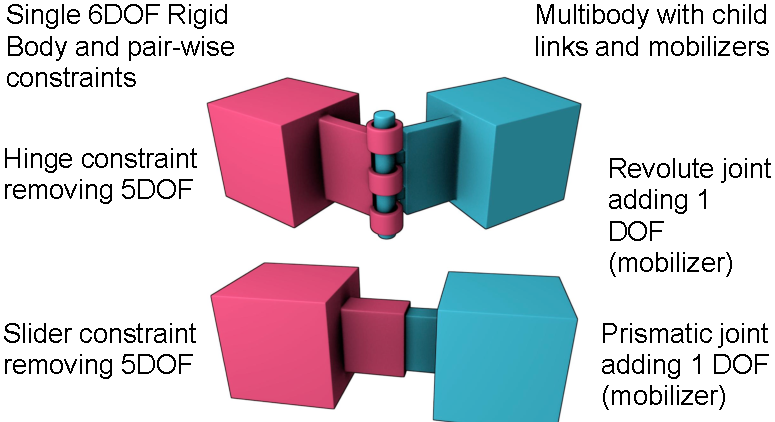
\includegraphics[width=0.8\textwidth]{Pictures/evolutionary-optimization/maximal-vs-reduced-coordinates.pdf}

\caption[Maximal vs. reduced coordinates]{Maximal vs. reduced coordinates. The text describes how a complex structure, and a hinge and slider constraint are represented in maximal (left) and reduced (right) coordinates. The Constrained Rigidbody Phenotype uses maximal coordinates, the Featherstone Multibody Phenotype uses reduced coordinates. Image from \cite{bib::Coumans2014}.}
\label{figure:maximal-vs-reduced}
\end{figure}

\subsubsection{Featherstone Multibody Phenotype}
\label{subsec:featherstone-multibody}

The Featherstone Multibody Phenotype is based on a fundamentally different concept called reduced coordinates or generalized coordinates (Figure \ref{figure:maximal-vs-reduced}). %
%
Reduced coordinates express only the degrees of freedom of each rigid-body relative to its parent body part, starting from each joint not having any DoFs. %
%
A simple hinge joint is then expressed as a 1-DoF revolute joint angle. Instead of constraint, as in the Constrained Rigidbody Phenotype, we call such a multibody joint a mobilizer. %
%
In the case of reduced coordinates, the position, velocity and acceleration are expressed with reference to the parent body part, meaning that we start to apply position and velocity updates at the root element and continue with the child body part. %
%
We also calculate the inertia of the whole hierarchy instead of only the inertias of the interacting body part when resolving body part-pairs. %
%
In the Featherstone representation, it is not necessary to resolve constraints, therefore we do not experience resolving forces and torques, thus no gaps exist between the rigid-bodies. %
%
The Featherstone representation, however, can not deal with circular structures \cite{bib::Coumans2014}, but such a feature was not needed in this simulation. %
%
This phenotype is very robust when it comes to hand-made as well as evolved phenotypes. %
%
That is why it is more suitable for evolving virtual creatures. 

\subsubsection{Model Organisms}

The model organisms are hand-coded genotypes to be developed into creatures that have specific properties. %
%
They are mainly used for testing and experimentation purposes, because they feature a non-redundant, simple genomic description and well-defined body part and joint descriptors.

\paragraph{Model Leg}

The model leg is a simple creature built from two equal body parts and one joint. %
%
The joint can be either set to a one DoF hinge joint or a three DoF spherical joint. %
%
The model leg's main purpose is to run experiments on chaotic controllers on a simple creature to observe the controller's behavior when changing gravity, restitution and friction.

\begin{figure}[H]
\centering
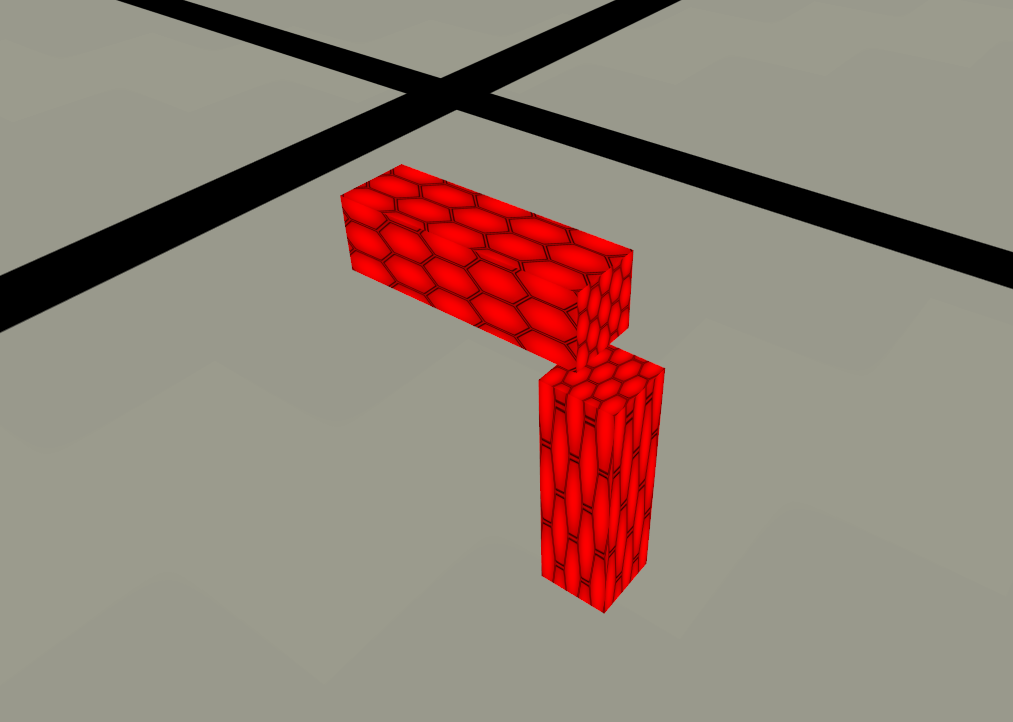
\includegraphics[width=0.32\textwidth]{model-organisms/Model-leg1.png}
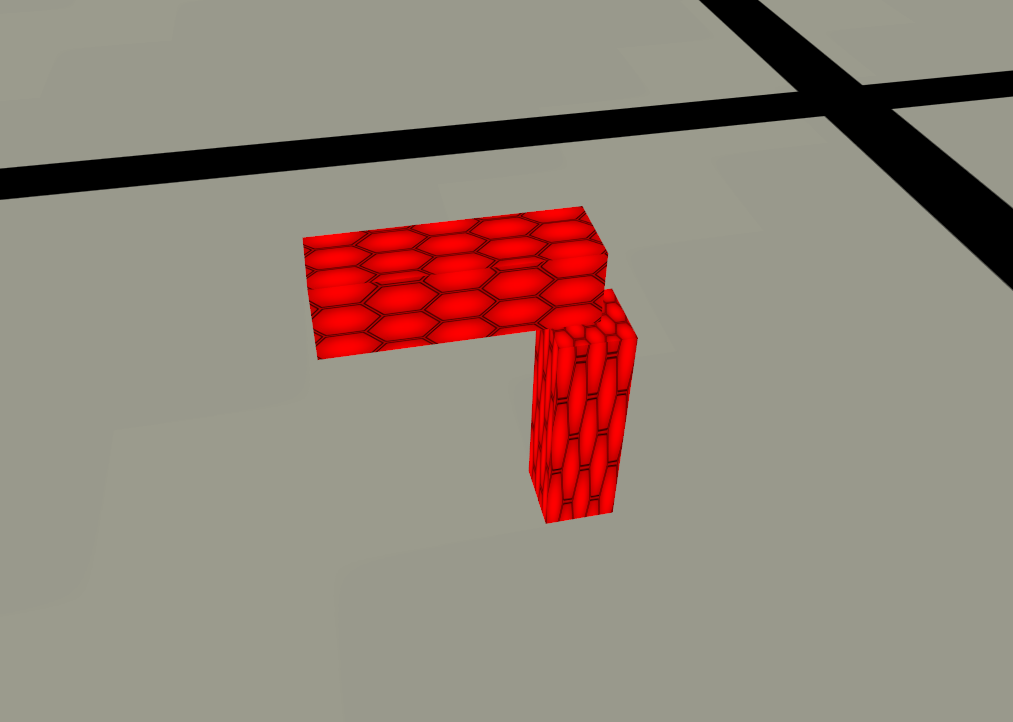
\includegraphics[width=0.32\textwidth]{model-organisms/Model-leg2.png}
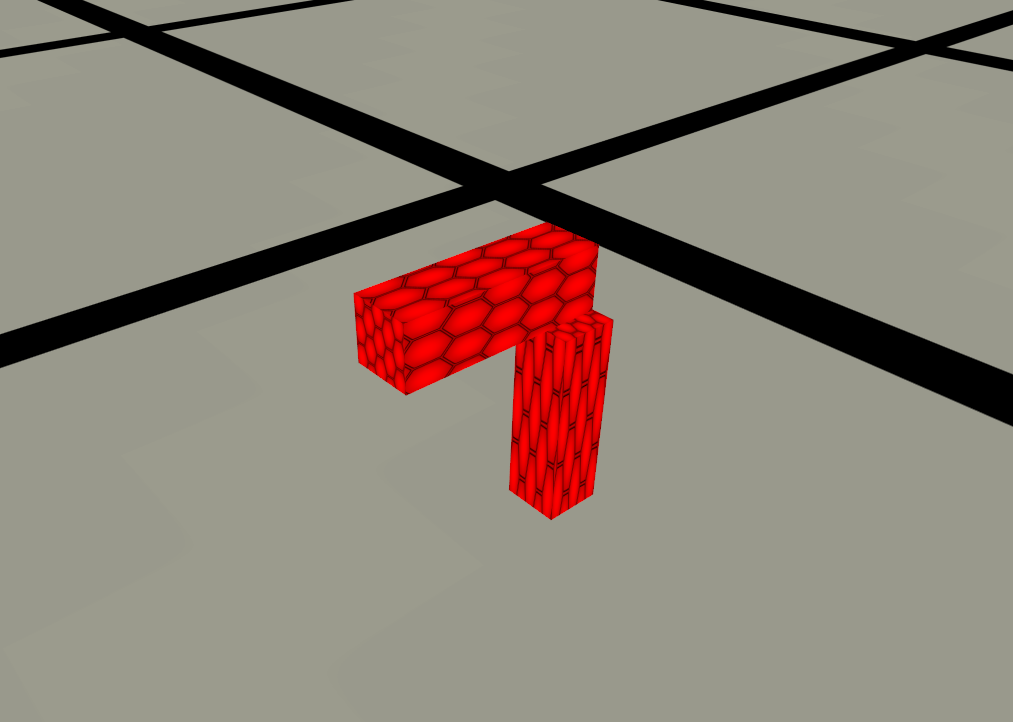
\includegraphics[width=0.32\textwidth]{model-organisms/Model-leg3.png}
\caption[The model leg]{The model leg, one of the model organisms of the Minemonics simulator. It features one single joint connecting two body parts.}
\label{figure:model-leg}
\end{figure}

\paragraph{Snake}

The snake is a creature built from a chain of equal body parts connected with one or three DoF joints similar to the model leg. %
%
In fact, the snake is just a chain of model legs with a higher number of body part-joint repetitions. 

\begin{figure}[H]
\centering
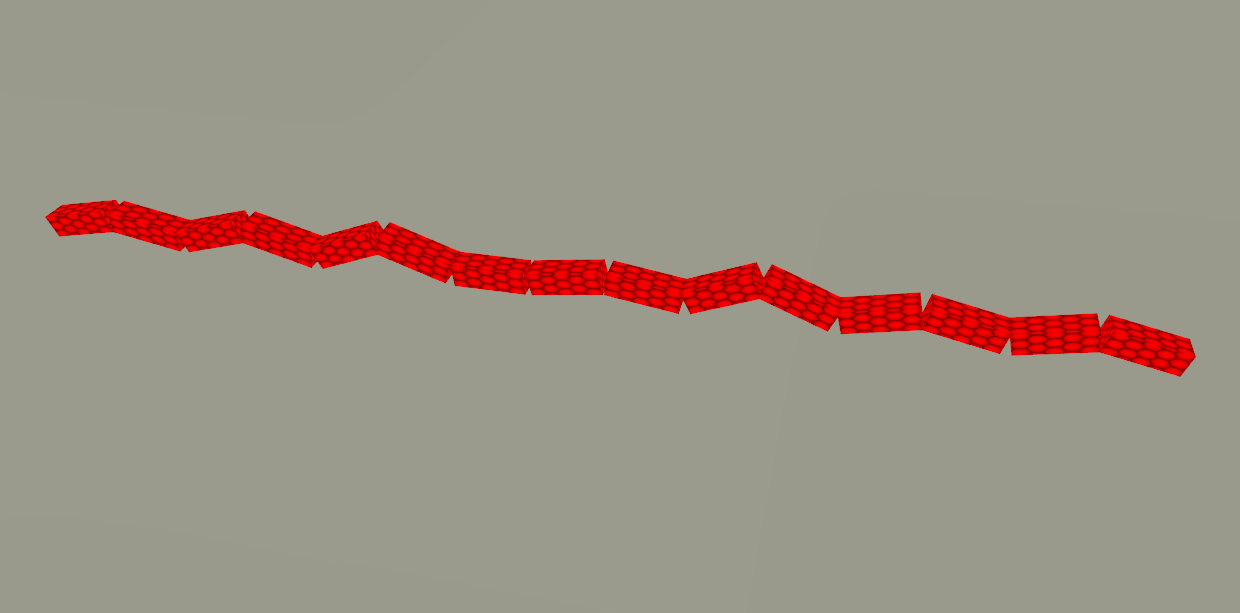
\includegraphics[width=0.32\textwidth]{model-organisms/Model-snake1.png}
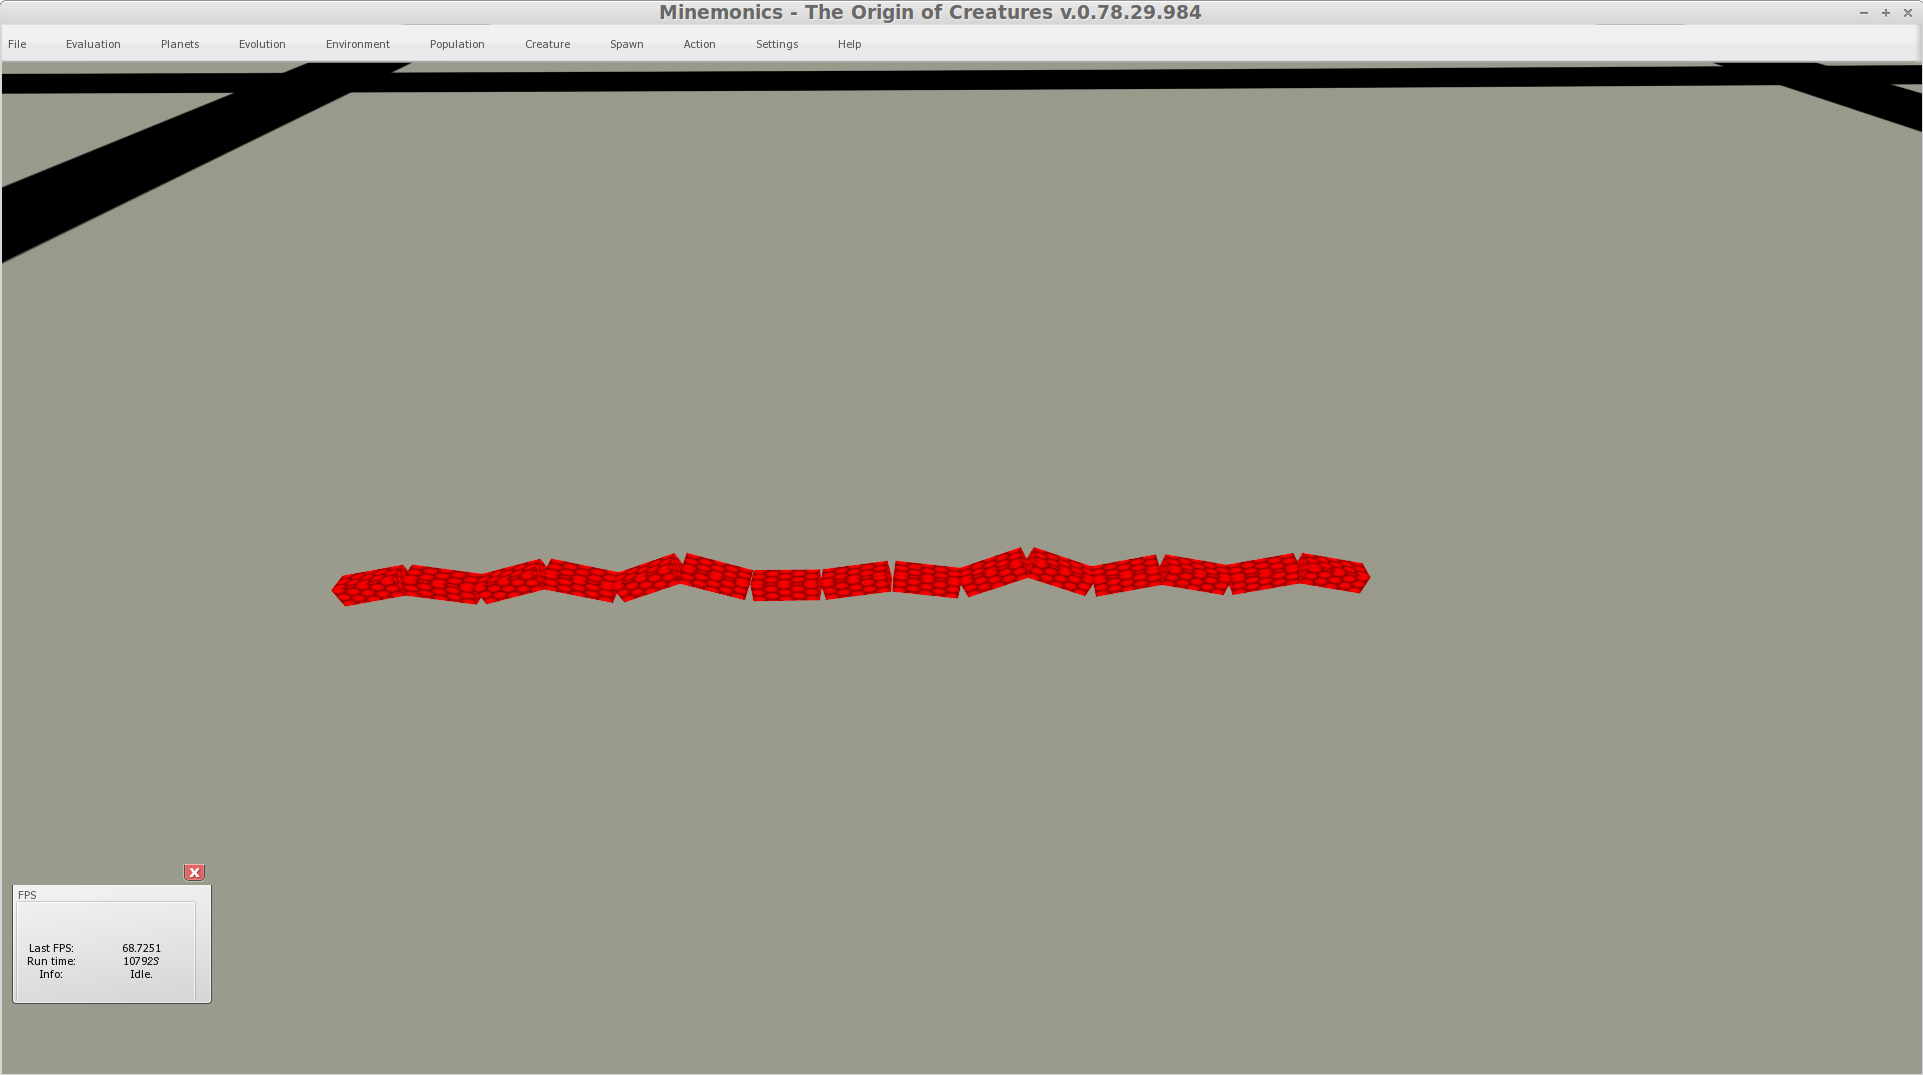
\includegraphics[width=0.32\textwidth]{model-organisms/Model-snake2.png}
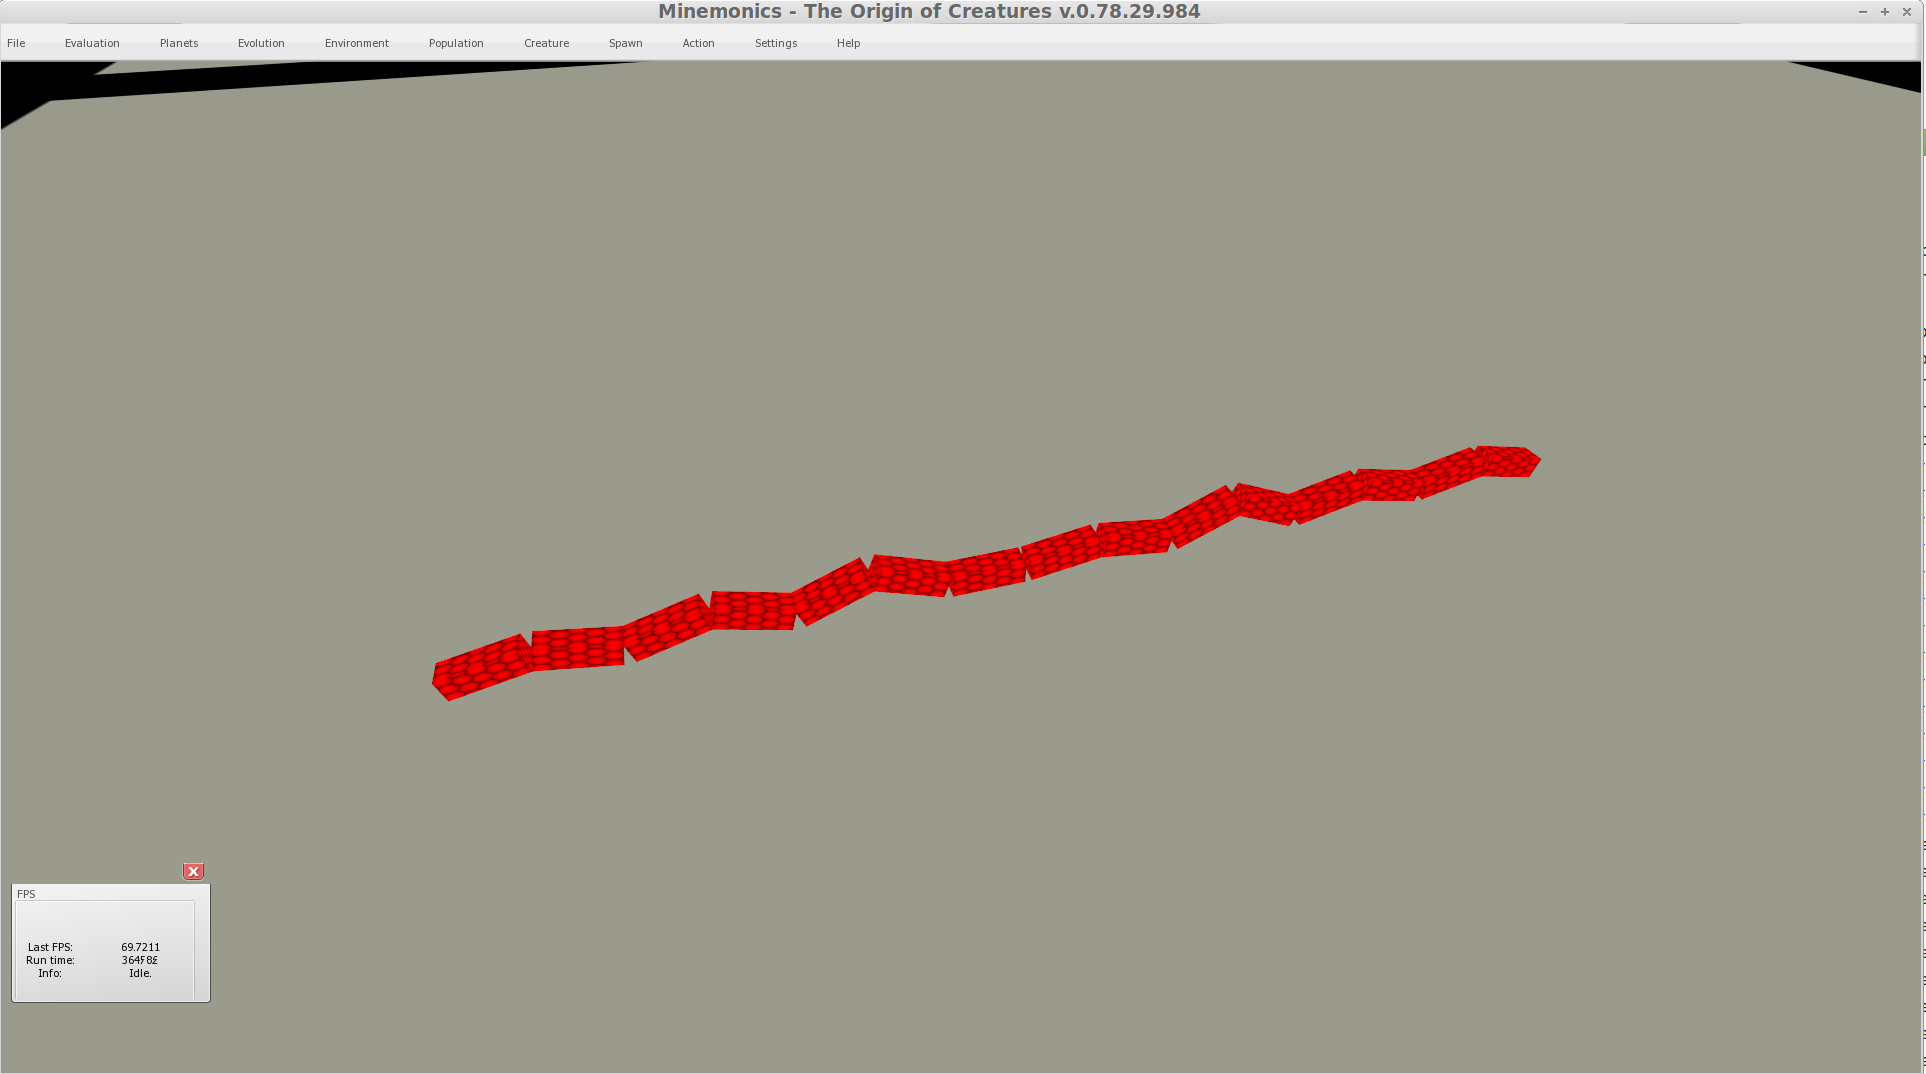
\includegraphics[width=0.32\textwidth]{model-organisms/Model-snake3.png}
\caption[The snake]{The snake. It features one long chain of body parts connected by either 1 DoF or 3 DoF joints.}
\label{figure:snake}
\end{figure}

\paragraph{Pod}

The Pod is a creature that can be configured to have a certain number of legs and a certain number of body elements. %
%
The main body is a body part on which the legs are attached in a circular manner. %
%
The number of legs is divided by the number of bodies, so that the same number of legs is attached to each body. %
%
With the same definition, its is possible to build insect-like creatures such as bugs, spiders, caterpillars and centipedes. %
%
It is mainly used to debug the Genotype-to-Phenotype transcription (Embryogenesis). %
%
Furthermore, experiments with a chain of chaotically oscillating controllers were run on it to see if patterns would emerge from it if the oscillators get coupled through the interaction with the ground.

\begin{figure}[H]
\centering
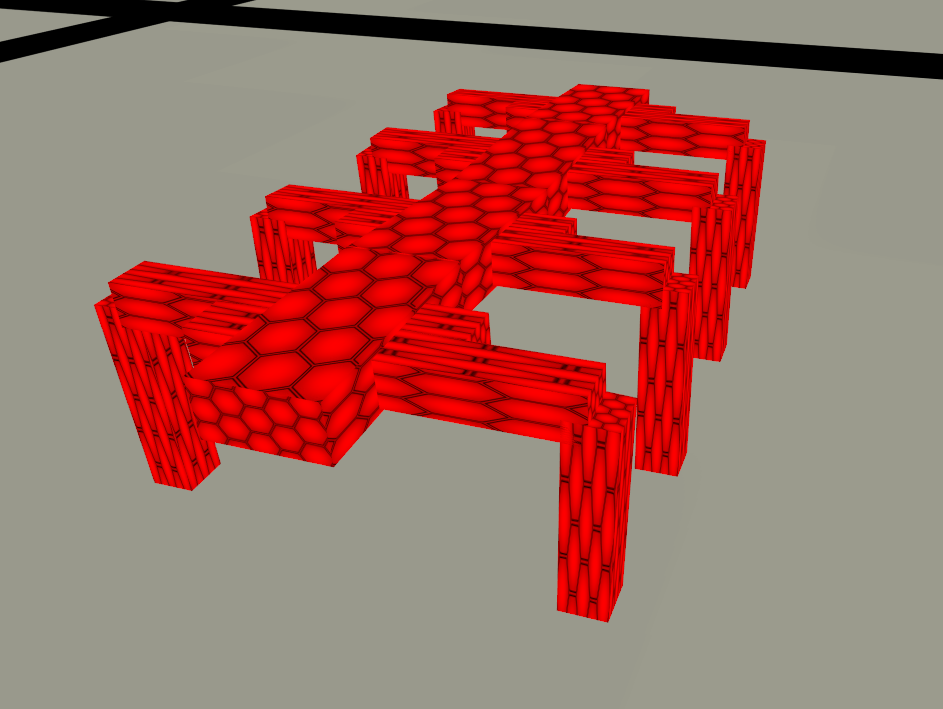
\includegraphics[width=0.32\textwidth]{model-organisms/Model-pod1.png}
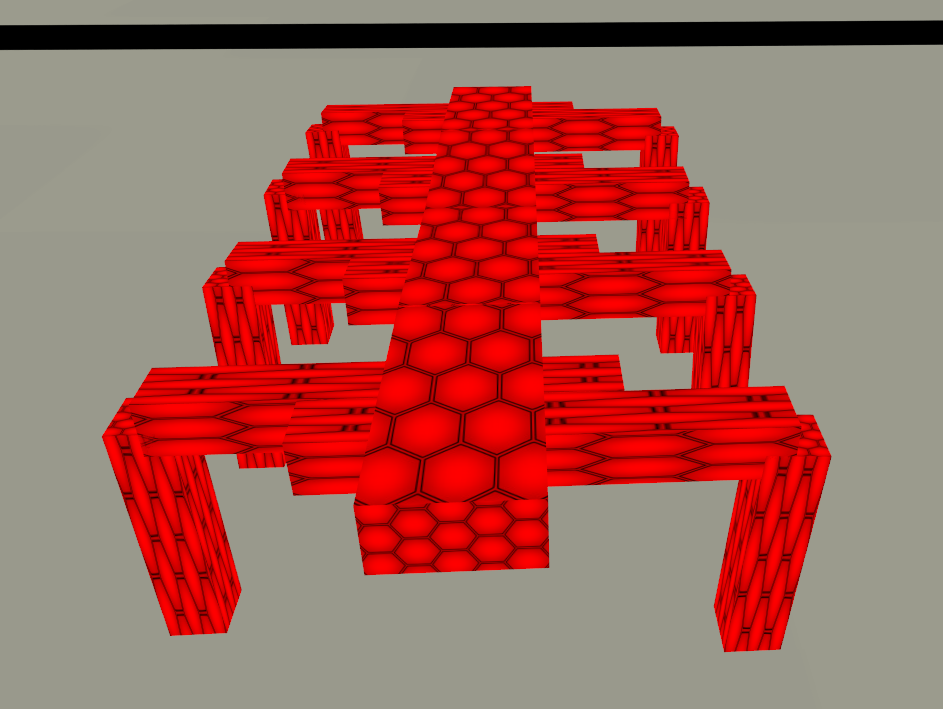
\includegraphics[width=0.32\textwidth]{model-organisms/Model-pod2.png}
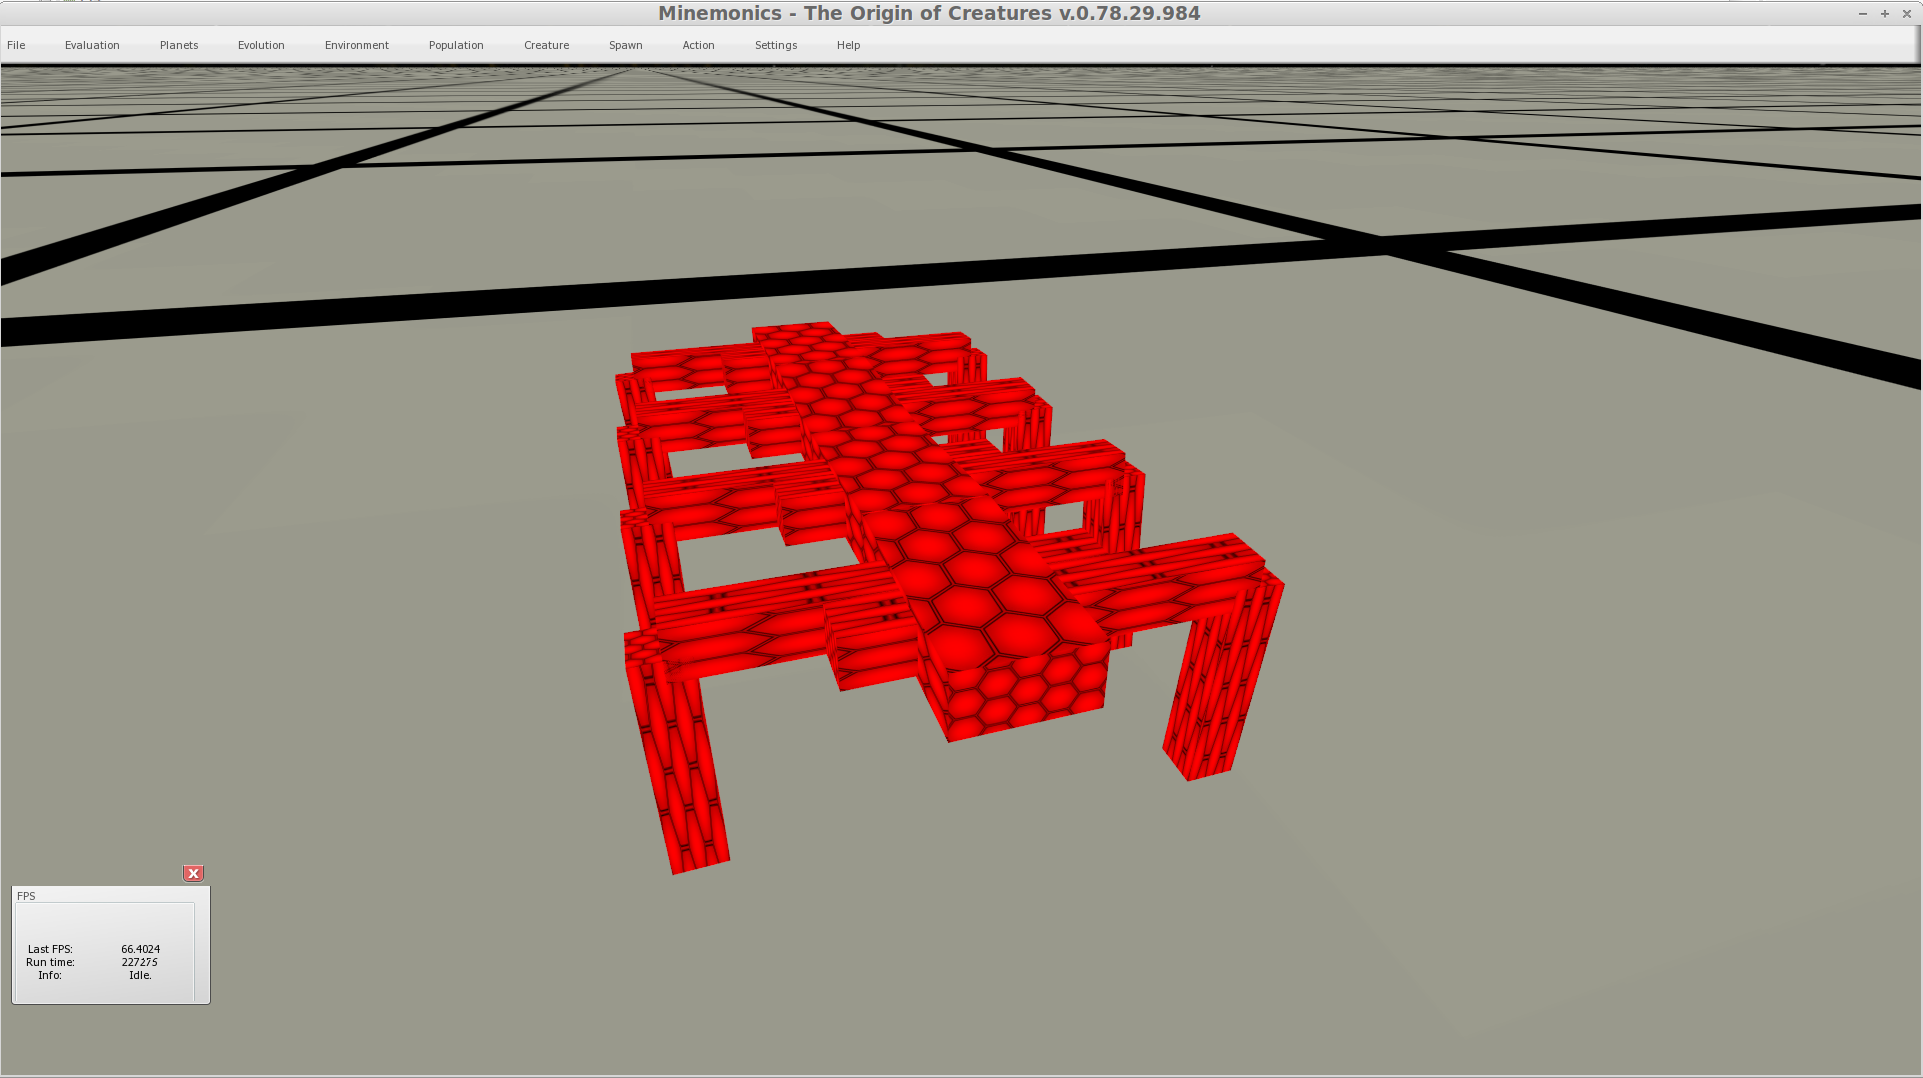
\includegraphics[width=0.32\textwidth]{model-organisms/Model-pod3.png}
\caption[The pod]{The pod is a basic structure that can be configured into having a certain number of main bodies and a certain number of legs. Thereby different morphologies such as hexapods or quadrupeds can be easily created.}
\label{figure:pod}
\end{figure}

\paragraph{Ragdoll}

The ragdoll blueprint produces a human-like form. %
%
It consists of differently configured joints and is mainly used to debug the Genotype-to-Phenotype transcription (Embryogenesis).

\begin{figure}[H]
\centering
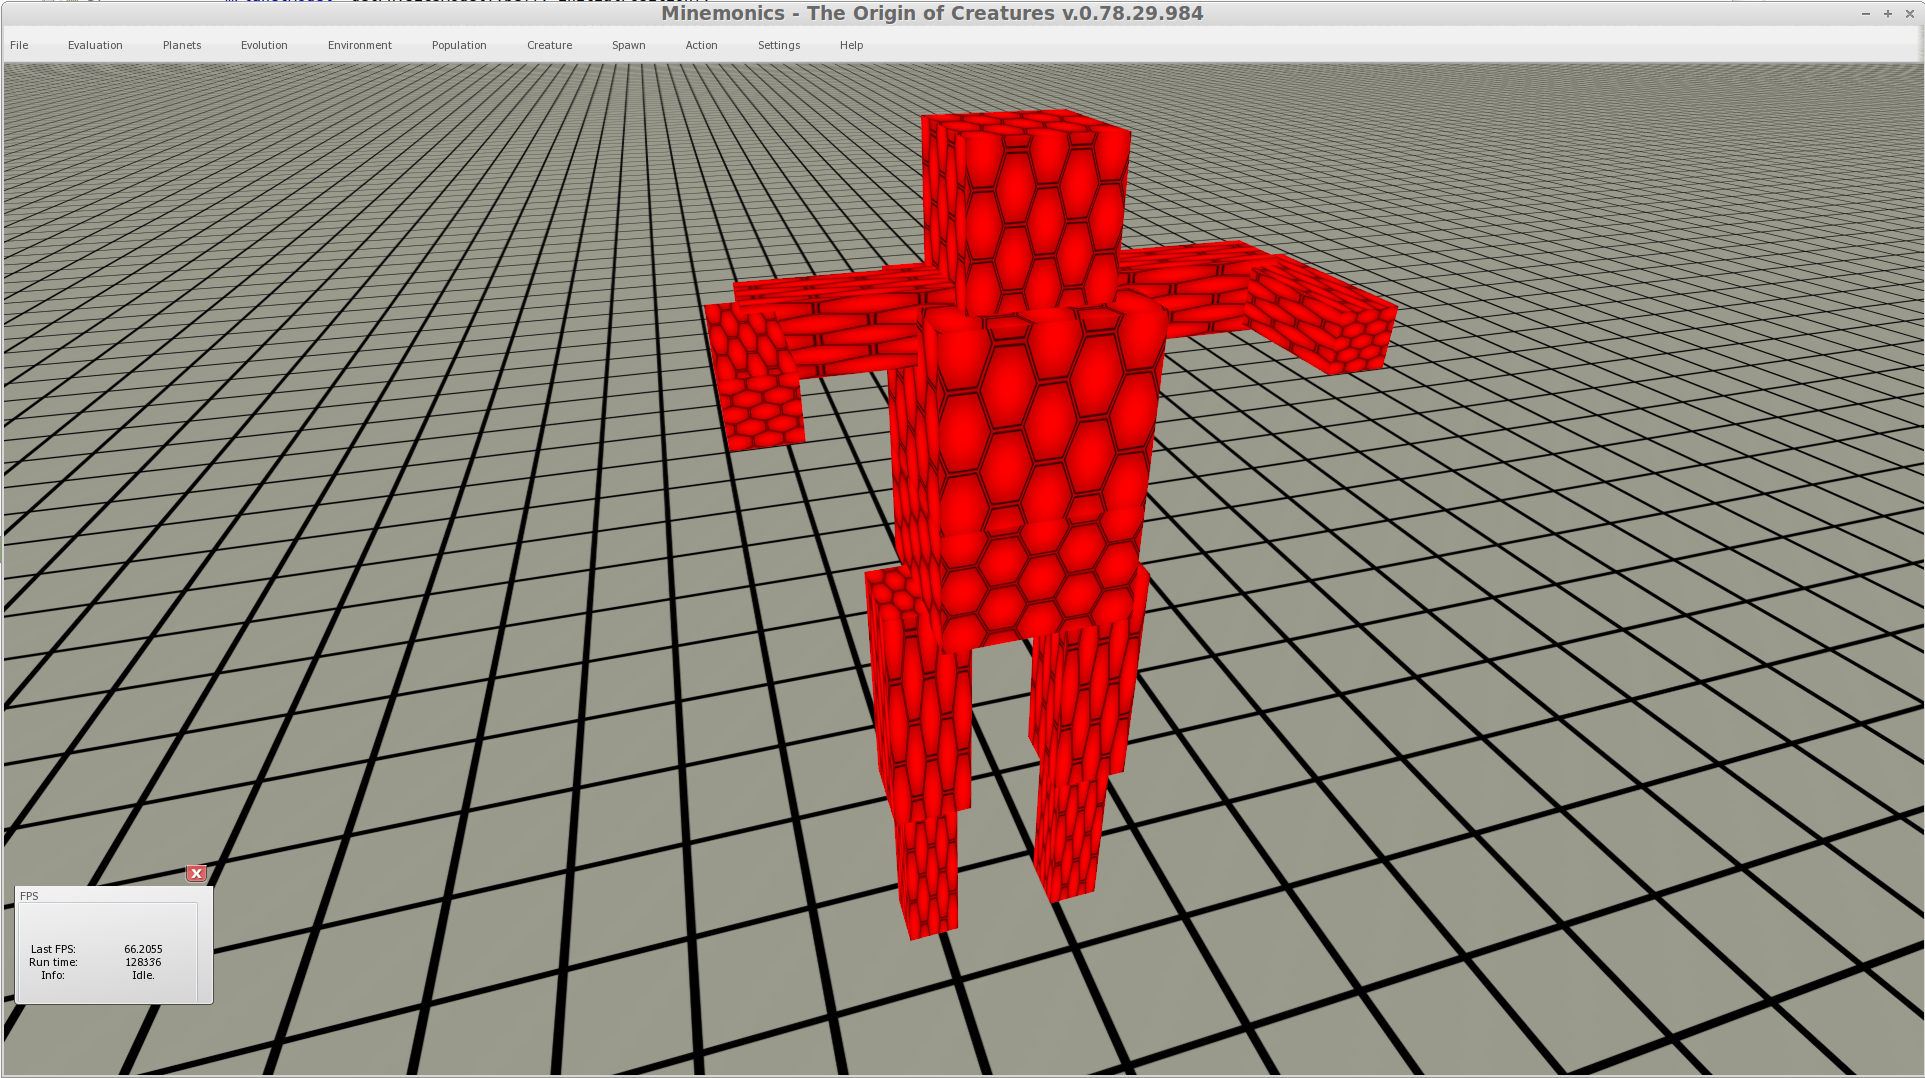
\includegraphics[width=0.32\textwidth]{model-organisms/Model-ragdoll1.png}
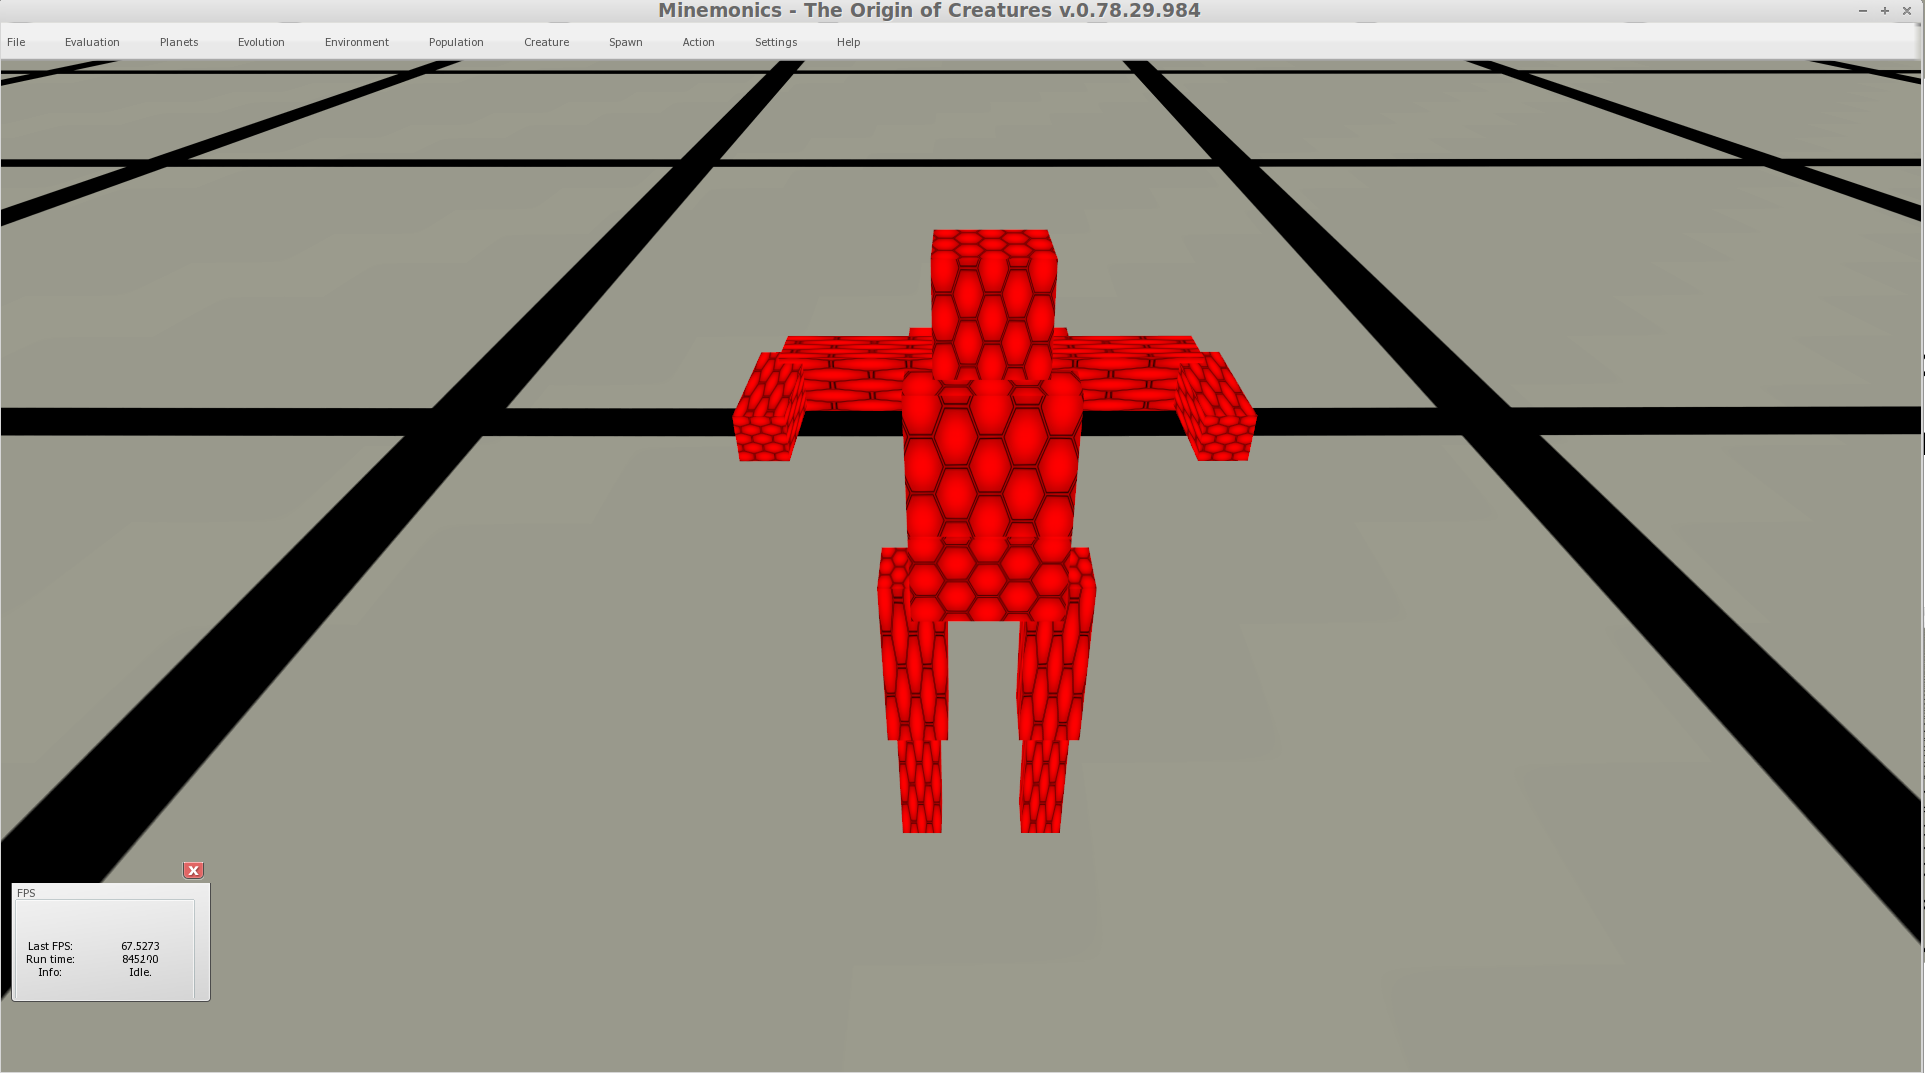
\includegraphics[width=0.32\textwidth]{model-organisms/Model-ragdoll2.png}
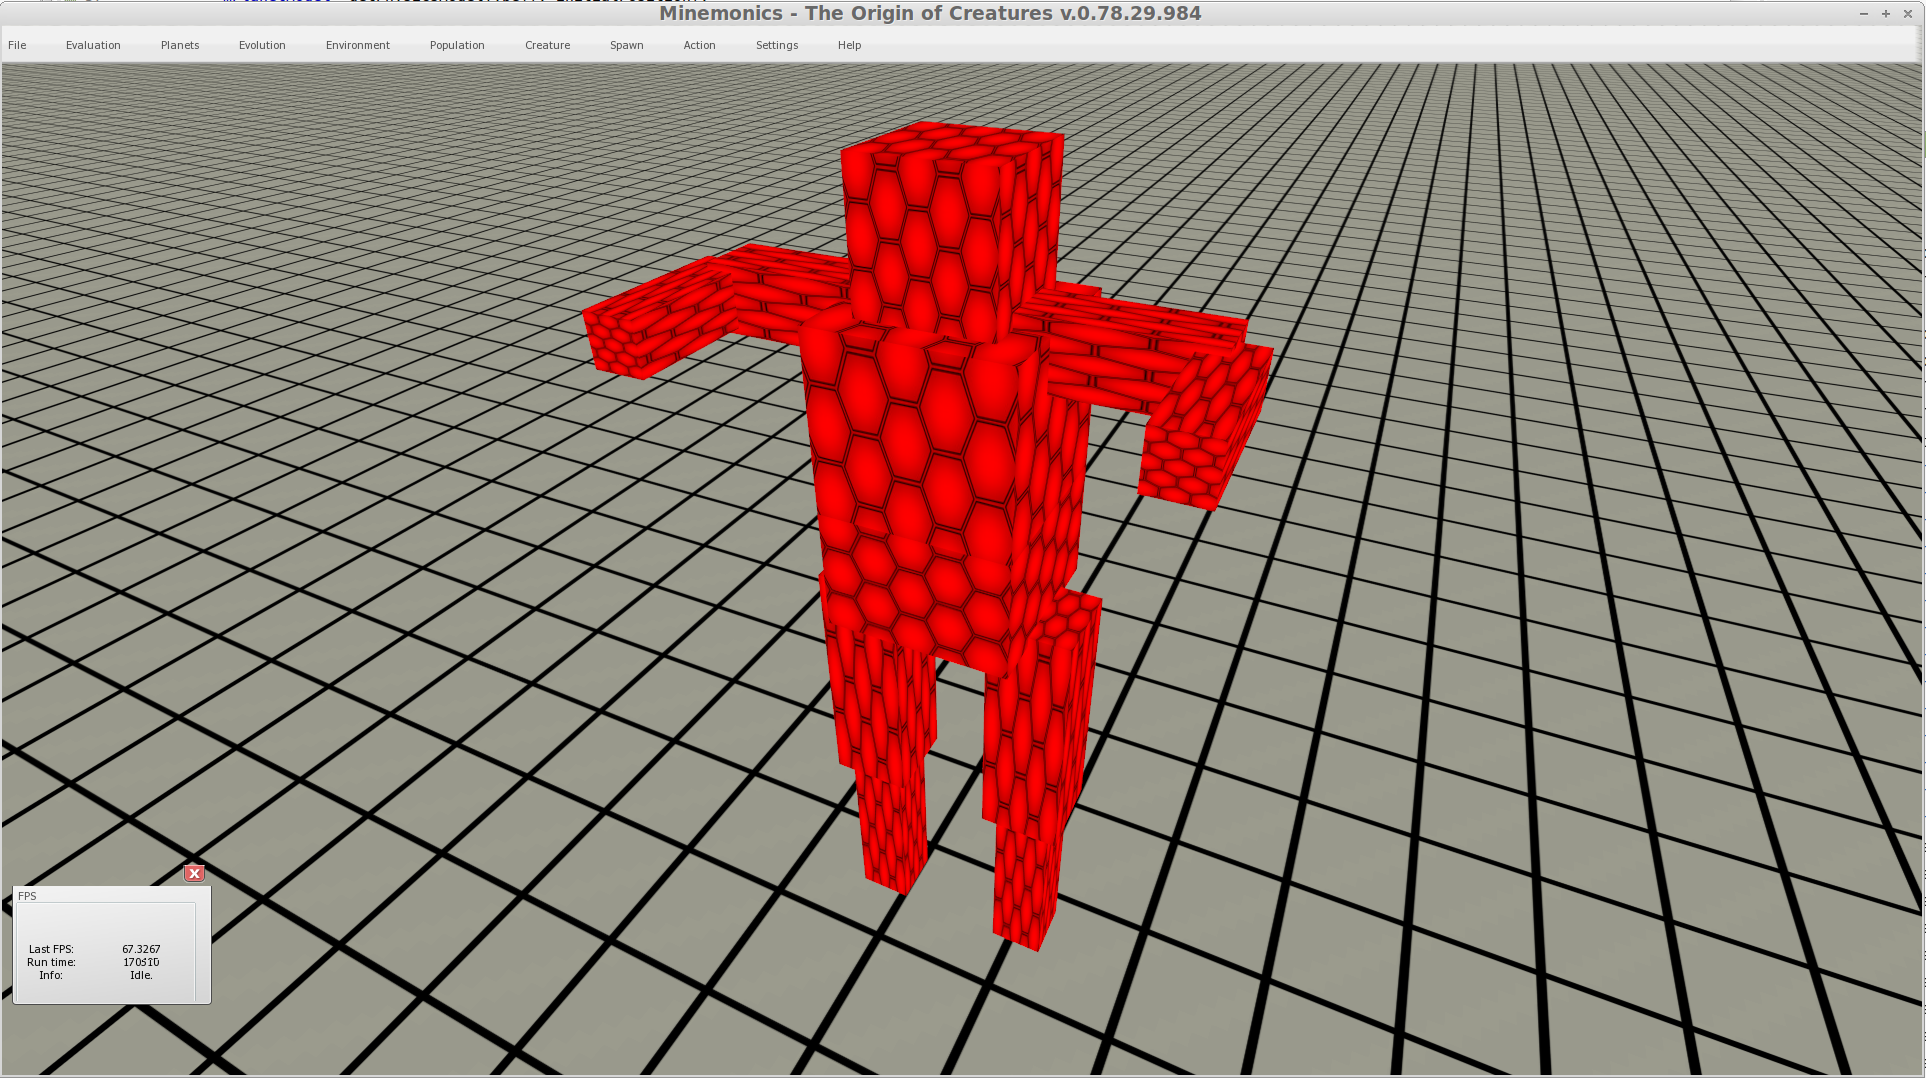
\includegraphics[width=0.32\textwidth]{model-organisms/Model-ragdoll3.png}
\caption[The ragdoll]{The ragdoll model organism. Its joints are differently configured so that errors during debug time of the Embryogenesis are revealed.}
\label{figure:ragdoll}
\end{figure}

\subsection{Embryogenesis}
\label{subsec:embryogenesis}

The Embryogenesis of a creature is a straight-forward process of transcribing a genotype into a phenotype. %
%
Starting from the root morphogene, the genome is expanded in a breath-first-search manner. %
%
This means that the process starts at the root node and transcribes the root's child nodes first, before moving on to the higher degree children. %
%
To store the intermediate results of the generation process, the Embryogenesis uses phenotype generators. %
%
Intermediate results are the morphogene branch of the parent morphogene and the parent body part element, the position and orientation of the current generation process, the current shrinkage factor of the generated body parts, if this is a flipped or mirrored branch, the length of the current root to leaf path and a list of the number of repetitions of different morphogene classes along this branch. %
%
The Embryogenesis is influenced by so called influence factors, which are propagated along the top-bottom path of the phenotype-tree. %
%
The influence factors, as mentioned before, are the flip and mirror flag of the morphogene branch and the current shrink factor, the maximum repetition limits, and the total number of body parts of the morphogene. %
%
The flip flag causes the embryogenesis to transcribe a top-bottom genome branch twice in the phenotype, once in its original form and once in flipped form. %
%
Flipping means that all positional and orientational definitions of the branch and following body parts are negated to create a second flipped version of the original genome branch. %
%
The mirror flag causes the embryogenesis to transcribe the genome branch twice in the phenotype, once in its original form and once a mirrored form mirrored the primary axis of the body part the branch is attached to. %
%
The current segment shrink factor shrinks all body part dimensions of the morphogene the branch points to and propagates along further branches of that morphogene. %
%
The maximum repetition limits, one per morphogene, permit or deny a further repetition of a body part along this top-bottom path of the phenotype tree. %
%
The total number of body parts causes the Embryogenesis stop when reached by the current body part quantity. %

The following pseudo code \ref{code:embryogenesis} describes the procedure of the embryogenesis. %

\begin{figure}[H]
\scriptsize
\textbf{Inputs:} Genotype \textit{genotype} of the individual\\
\textbf{Result:} Fully developed morphology and controller of the creature
\begin{PseudoCode}[otherkeywords={create,add,exit,build,append,place,get,each},emph={rootMorphogene,genome,generatorsList, phenotypeGenerator,segmentsDepthLimit,currentBodyPartQty,childBodyPart,generator,morphogeneBranch,phenotypeGenerators,genotype,parentBodyPart,morphogene,.,maxBodyPartQty,morphogeneBranches,branch,joint,controller,orientation,baseOrientation,repetitionsList},emphstyle={\bfseries\textit}]
get rootMorphogene from genotype
phenotypeGenerator.morphogene = rootMorphogene
phenotypeGenerator.segmentsDepthLimit = 0
currentBodyPartQty = 0
phenotypeGenerator.baseOrientation = Identity
phenotypeGenerator.repetitionsList = {}
add phenotypeGenerator to generatorsList

while generatorsList is not empty
	get generator from generatorsList
	
	exit if generator.segmentsDepthLimit = genotype.segmentsDepthLimit or currentBodyPartQty = genotype.maxBodyPartQty
	
	build new childBodyPart according to generator.morphogene, generator.flipped and generator.mirrored
	
	if childBodyPart has to be attached to a parentBodyPart
		append childBodyPart to parentBodyPart
		build joint & controller according to generator.morphogeneBranch

	rotate generator.baseOrientation with childBodyPart.orientation
	
	get morphogeneBranches from generator.morphogene
	
	for each branch in morphogeneBranches
		if branch.morphogene not exhausted in generator.repetitionsList
			create new phenotypeGenerator or multiple if branch is flipped or mirrored
			copy phenotypeGenerator settings from generator
			phenotypeGenerator.segmentsDepthLimit += 1
			phenotypeGenerator.repetitionsList[branch.morphogene] += 1
			phenotypeGenerator.morphogeneBranch = branch
			add phenotypeGenerator to generatorsList
		
	currentBodyPartQty +=1
\end{PseudoCode}
\caption{Developing a creature using Embryogenesis}
\label{code:embryogenesis}
\end{figure}

\subsection{Reaper}
\label{subsection:Reaper}
% rev. 2

At the end of all evaluations for a certain population's generation, the simulation arrives at the evolution step. %
%
In the evolution step, the following operations are performed by the reaper: Culling a percentage of the worst performing creatures according to the total fitness ranking, variation of the remaining creatures with different variance operators according to the respective percentages and sowing of new creatures partly from crossover and random generation. %
%
In the Minemonics simulator, \unit[30]{\%} are culled first. The remaining creatures are equally distributed among the variation operations Gene specification, Gene split, Gene purge, Branch specification, Grow stub gene and graft feature mutation, another equal share from the fittest creatures is left untouched following an elitism strategy. Then the missing \unit[30]{\%} are replaced with equal amounts of creature generated by crossover and randomized instantiation.

In the following sections, the different operations are described in detail.

\subsubsection{Culling}
\label{subsubsection:Culling}

In order to cull individuals from the population, the individuals first have to be sorted according to their fitness. %
%
For a single fitness function, the sorting is straight forward. %
%
But in many cases, it is necessary to have individuals adapt to multiple fitness functions to represent the desired fitness landscape. %
%
Furthermore, one fitness condition might have a higher weight than the others.. %
%
It is hard to combine different fitness functions, usually because it is not possible to adjust them to the same scaling, especially if one is considered better with decreasing values. %
%
Therefore, competitive ranking was chosen to combine the fitness functions. %
%
This means that for each fitness function, the individuals are sorted according to their respective fitness value and a score is assigned to each rank (in the simulator, the score for a rank is the number of individuals that performed worse). %
%
Then, for each individual $c_n$ for $m$ fitness functions, the scores $r_i$ multiplied by the respective fitness function weights $w_i$ are summed. 

\[\text{fitness score}_{c_n} = \sum\limits^m_{i=1} r_i \cdot w_i \]

Finally, the individuals are sorted by their fitness score, which results in their total ranking according to their fitness. %
%
Unfortunately, by this procedure, the score loses the information whether the best individual of the creature increased its fitness. %
%
However, this can easily be found out by logging all fitness function values of the best creature of the population at the end of the evaluation.

\subsubsection{Crossover}
\label{subsec:crossover}
% rev. 2

The typical crossover strategy inspired by biological crossover is commonly known as cutting the two parent genomes into segments and then recombining segments of the parents into a new valid genome. %
%
This section additionally describes the procedure of how to choose matching parents.

Using the creatures sorted by the fitness ranking, a percentage of those best performing creatures are chosen to be possible parents. %
%
To create new offspring, from every possible parent a number of offsprings is generated. %
%
The number of offspring per parent is found by diving the total number of new creatures to be created by crossover by the number of parents. %
%
Having found one of the parent, the other parent is chosen as follows: With \(\unit[50]{\%}\) chance, the parent is chosen as one from a tournament of 10, where the best creature of that tournament is chosen as the second partner. %
%
Each tournament creature is drawn from the population using a normal positive integer distribution such that the index of the first creature has the highest probability to be chosen and the \(\sigma\) is such that the probability decays nearly completely that the index of the last creature is chosen. %
%
With the remaining \(\unit[50]{\%}\) chance, the second parent is chosen at random from the population.

The actual crossover process is very similar to the commonly known one. %
%
From the genomes of each parent a subsegment is taken and the second is directly appended to the first one. %
%
Unlike the process in classical bit-array notions of genomes is that the two segments have to be interconnected with branches in order to be properly combined. %
%
Therefore 10 random branches are mutated such that they interconnect the two subsegments and all gene branches are repaired to reset all invalid branching indices.

\subsubsection{Grafting}
% rev. 2

Grafting is similar to crossover in terms of finding two partners (the first called the donor, the second called the receiver), but does not produce offsprings. %
%
Instead of just cutting both genomes at random positions and recombining them, it picks a random morphogene in the donor genome and copies this morphogene and its children over to the receiver genome until a certain copying depth $x$ is reached, where $x \in [5,10]$. %
%
As the name says, the idea of this mutation is to copy functional segments to transfer an evolved feature from one creature to another. %
%
The functional segments could for instance represent a specific leg or main body structure.

\subsubsection{Mutations}
% rev. 2

All other variational operators work on single elements of a single genome. %
%
The mutations modify specific aspects of the genome and are specifically made for the genomic structure.

\paragraph{Gene Specification Mutation}

The gene specification mutation applied to a genome iterates over all its morphogene classes. %
%
For each class, with probability $0.2$, the morphogene is reinitialized with random values. %
%
This affects all values except for the morphogene branches which stay unchanged.

\paragraph{Gene Split Mutation}

The gene split mutation applied to a genome iterates over all morphogene classes. %
%
For each class, with probability $0.2$, the morphogene is split along the X, Y or Z axis into two morphogenes occupying roughly the same total volume as the original body part. %
%
The morphogenes are then connected with a single branch representing a completely limited joint.

\paragraph{Gene Purge Mutation}

The gene purge mutation applied to a genome purges a gene by mutating it. %
%
Then it iterates over all other morphogenes and deactivates all morphogene branches pointing to the gene to be purged. %
%
Thereby the purge gene belongs to the non-expressing part of the genome and is therefore purged.

\paragraph{Branch Specification Mutation}

The branch specification mutation applied to a genome iterates over all morphogene classes. %
%
For each class, with probability $0.2$, a random morphogene branch is chosen and is reinitialized with random values. 

\paragraph{Grow Stub Gene Mutation}

The grow stub gene mutation applied to a genome iterates over all morphogene classes. %
%
For each class, with probability $0.6$, $x$ new branches are added to the morphogene, where $x \in [0,2]$. %
%
The branches reconnect the stub gene to others and therefore increase the interconnectivity of unconnected morphogene classes.

\section{Evolutionary Cycle}
% rev. 1

To describe how the different components play together, an example evolutionary cycle of one planet with a flat plane environment and a population of 10 individuals is outlined. %
%
One evolutionary cycle can be separated into 2 substeps, the evaluation step and the variation step. %
%
Before the cycle can begin, the planet and its environment are set up, the (infinite) flat plane is positioned at the origin of the coordinate system, and each randomly generated individual's genome is transcribed into a phenotype by the Embryogenesis. %
%
The population is not yet visible anywhere and awaits evaluation.

\subsection{Evaluation Step}
% rev. 2

During the evaluation step, each individual is dropped into the simulation slightly above the ground for the selected evaluation period of usually 20 seconds. %
%
In single creature mode, which was used for all experiments, every creature is evaluated separately. %
%
If a creature consists of zero or only one body part, the creature is discarded, since it is degenerate and can not move at all, therefore is worthless to be evaluated. %
%
Furthermore, the evolution discards creatures that produce very high joint velocities, which is usually an indication that the creature might exploit unrealistic physical forces. %
%
During the evaluation of the other creatures, the juries evaluate the performance and calculate the combined fitness value at the end of the evaluation. %
%
If all evaluations are over, the evolution switches to the variation step.

\subsection{Variation Step}
% rev. 2

During the variation step, the reaper picks up the population and culls the worst performing creatures. %
%
Leaving a top percentage of creatures without variation (Elitism), it produces offspring by crossover based on the elite and an additional partner, then applies the mutations to the rest of the population. %
%
Finally it replaces the remaining number of missing creatures with new, randomly generated creatures.

\subsection{Simulator Specification}

The simulator was developed in C++ using a Graphics Engine called Ogre3D \cite{bib:Ogre3D}, a GUI engine called CeGUI \cite{bib:CEGUI} and a Physics engine called Bullet Physics \cite{bib:BulletPhysics2015}. %
%
Additionally, the boost library \cite{bib:Boost} was used to speed up the development of logging data and the creature serialization to disk. %
%
The simulator features a rich interface, which can be manipulated using the mouse and the keyboard. Using the graphical interface's menu, a new planet can be configured and instantiated, then a population can be configured and added to it. %
%
Furthermore, the gravity of the current planet can be changed to different predefined gravitational values of our solar system. %
%
During the evaluation, the evaluation speed can be changed and the simulator can be run in headless mode, meaning that the graphical output is omitted to speed up the simulation. %
%
Moreover, the user can move within the simulated space to look at the creature from different angles and can manipulate the creature using the mouse. %
%
To observe the current controller and joint dynamics, a window with two graphs can be opened, plotting 50 time steps of the internal states in real-time. %
%
If a currently evaluated creature gets stuck in the evaluation or is visibly not fit to be considered, the creature can be culled manually. %
%
To look through the evaluated creatures, a population can be loaded and can be sorted out by manually saving some of the creatures and culling others without saving. %

\begin{figure}[H]
\centering
\hspace*{-6em}
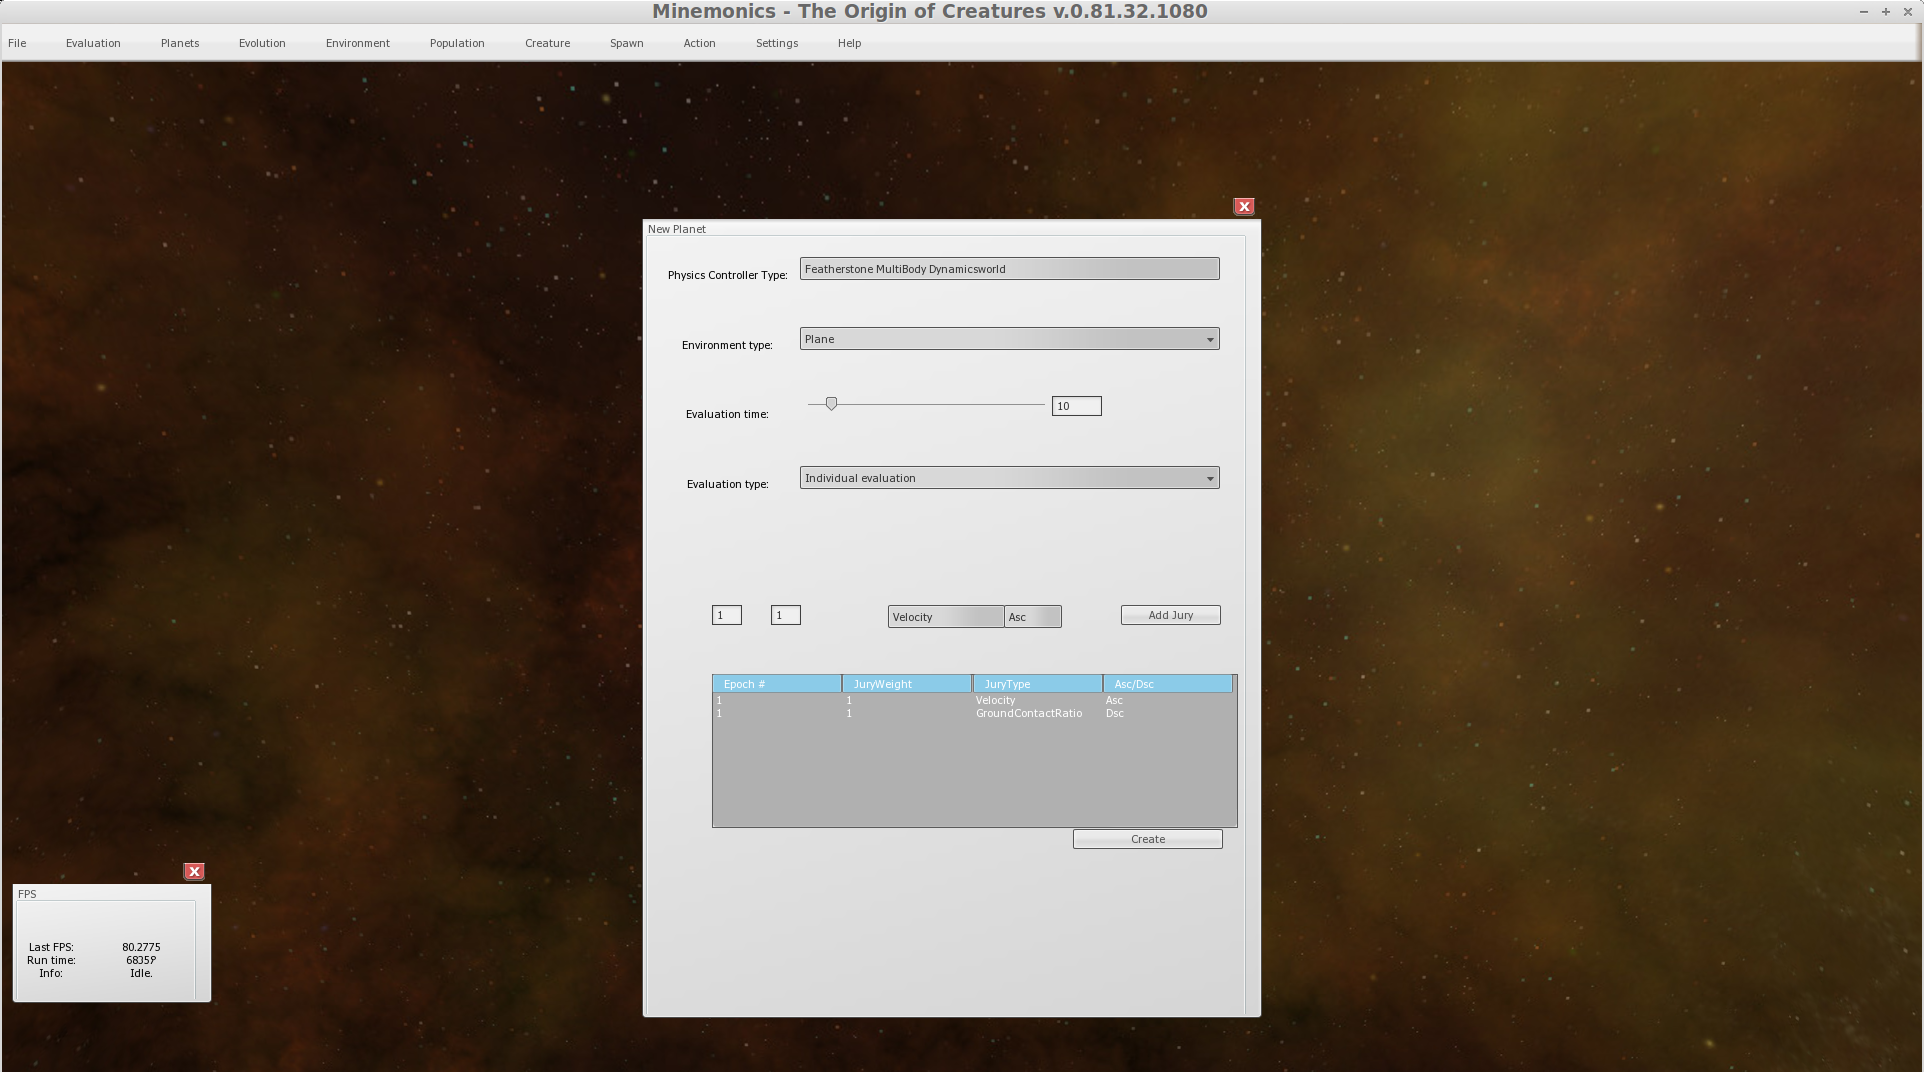
\includegraphics[width=1.2\textwidth]{evolutionary-optimization/planet-configuration.png}
\caption[The simulator planet configuration interface]{The figure shows the interface of the simulator when configuring a new planet. In the lower part of the configuration window, the configured juries can be seen.}
\label{figure:simulator-planet-config}
\end{figure}

\begin{figure}[H]
\centering
\hspace*{-6em}
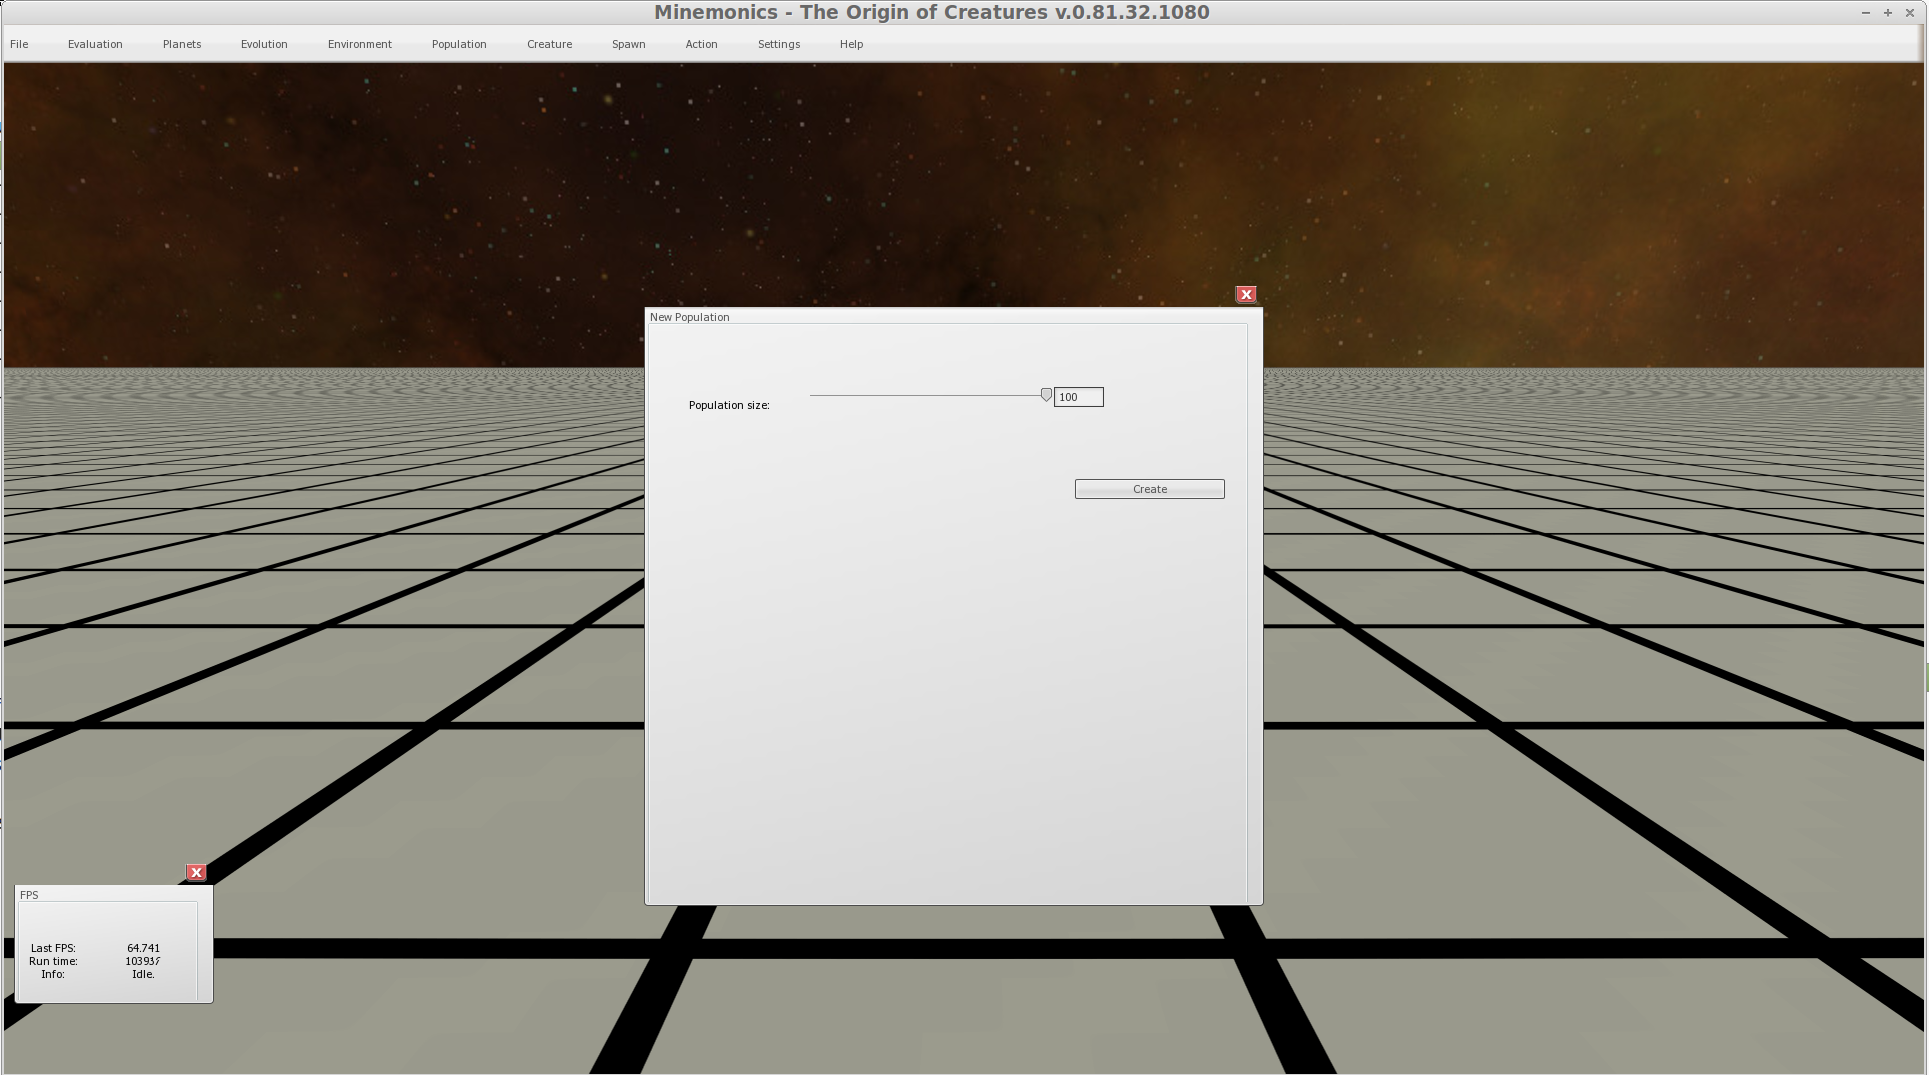
\includegraphics[width=1.2\textwidth]{evolutionary-optimization/population-configuration.png}
\caption[The simulator population configuration interface]{The figure shows the interface of the simulator featuring when configuring a new population.}
\label{figure:simulator-population-config}
\end{figure}

\begin{figure}[H]
\centering
\hspace*{-6em}
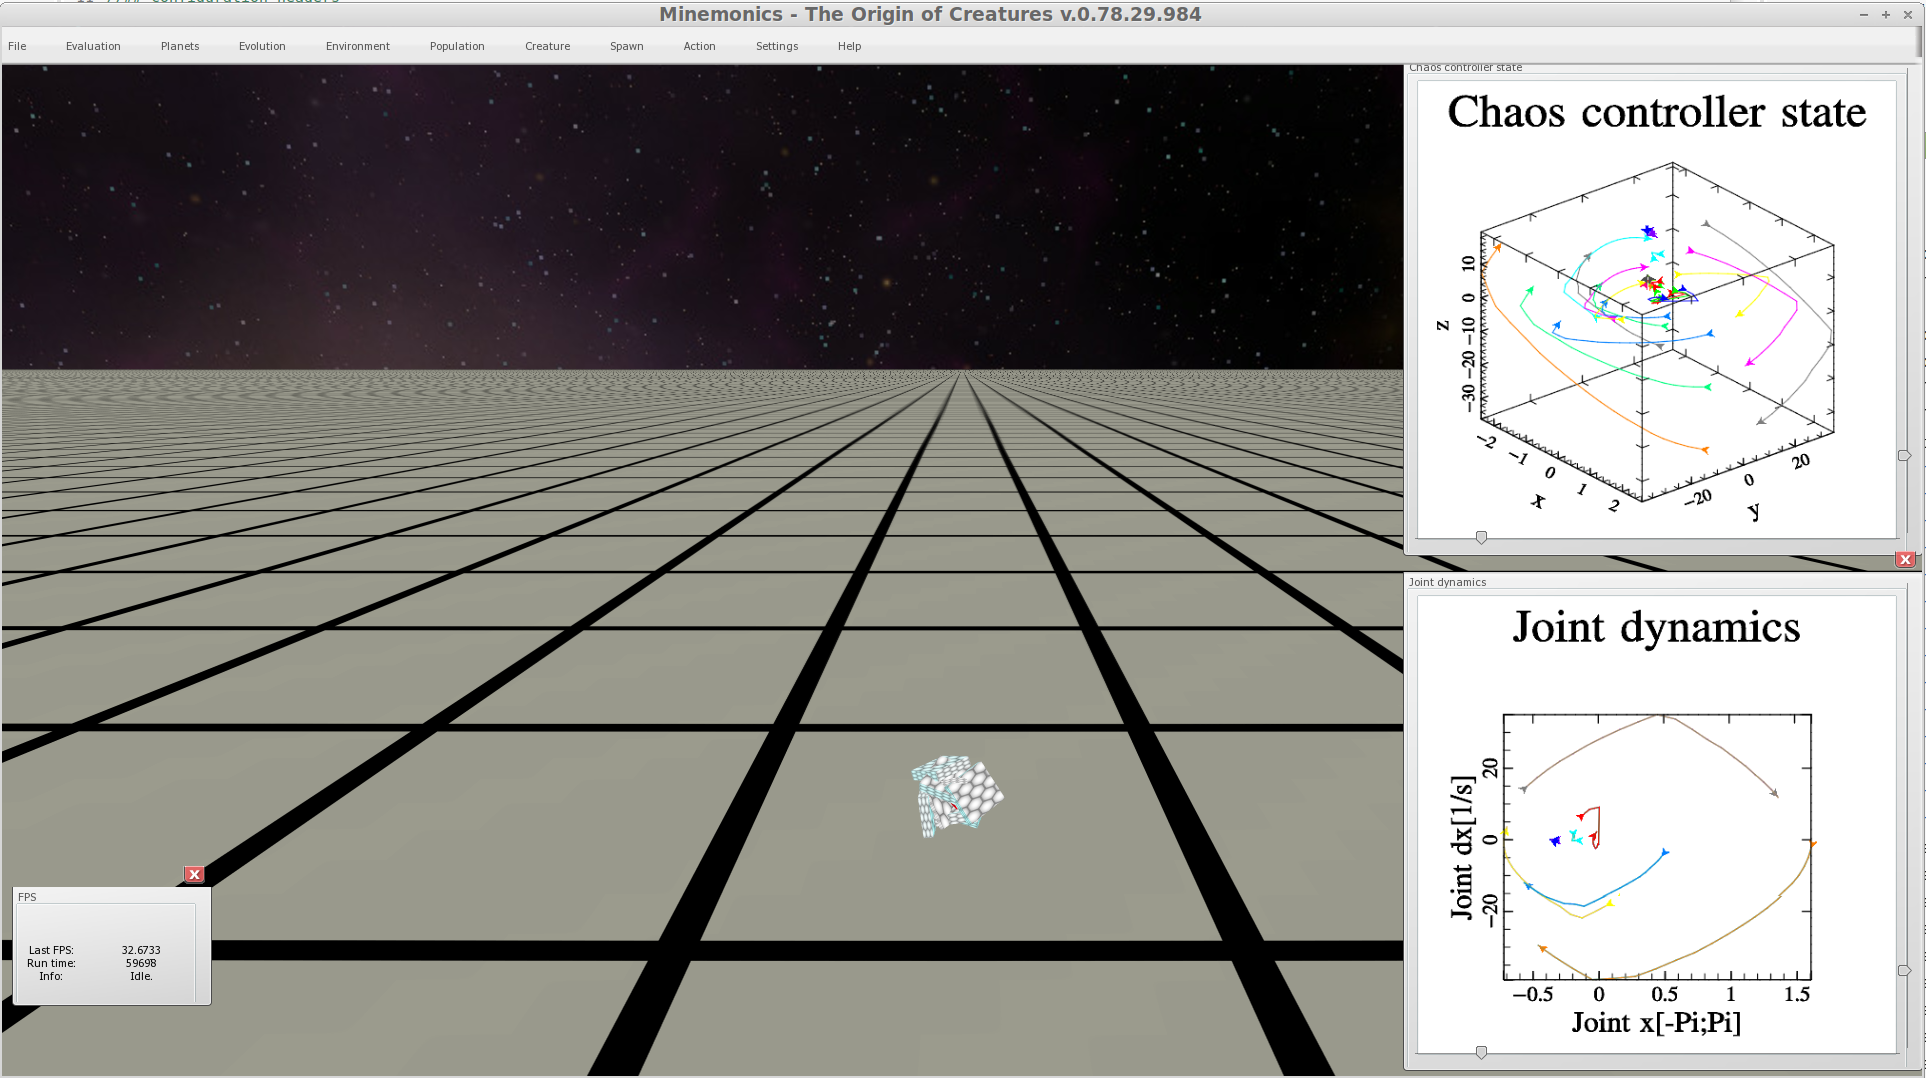
\includegraphics[width=1.2\textwidth]{evolutionary-optimization/simulator2.png}
\caption[The simulator evolution interface]{The figure shows the interface of the simulator featuring a creature in evaluation. On the right-hand side, the window showing the internal graph state can be seen.}
\label{figure:simulator}
\end{figure}

\begin{figure}[H]
\centering
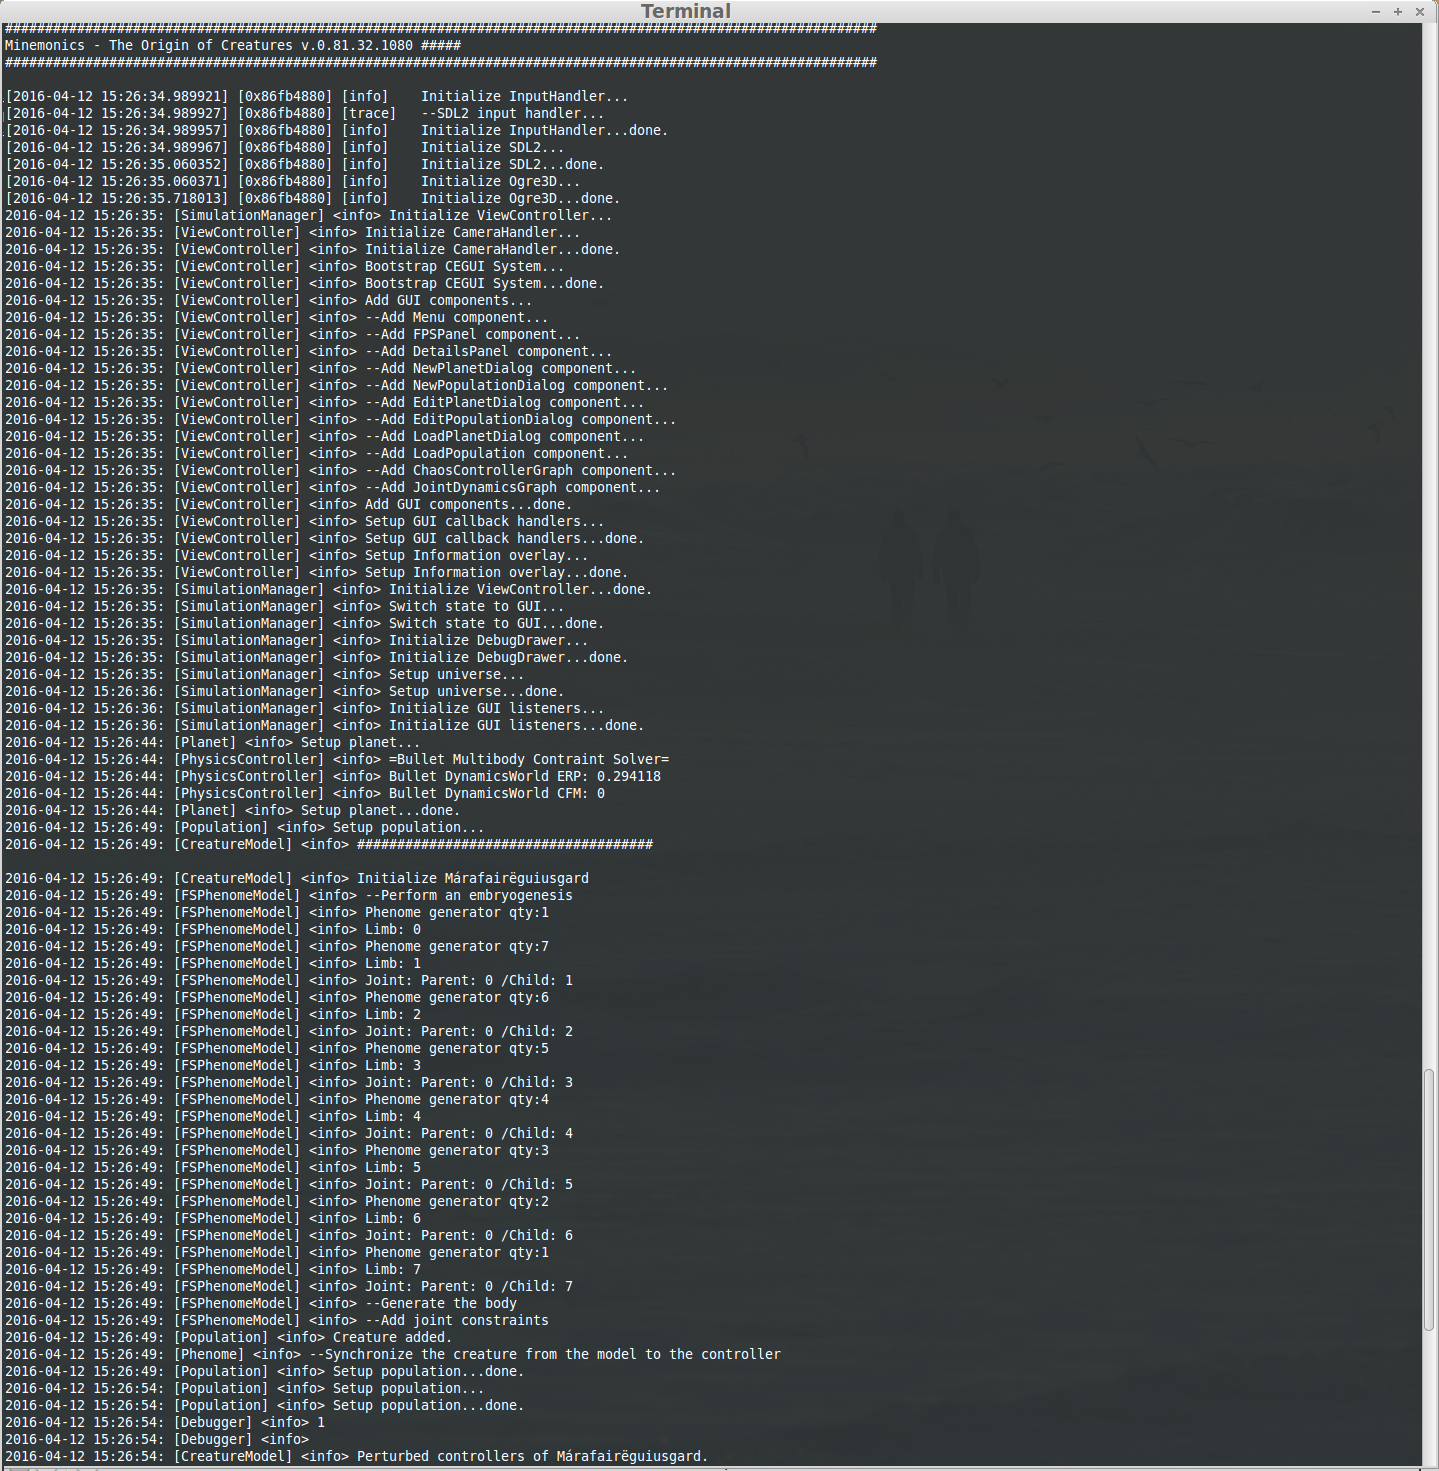
\includegraphics[width=0.73\textwidth]{evolutionary-optimization/terminal-output.png}
\caption[The simulator terminal output]{The figure shows the simulator's terminal output providing general information to the running evolutionary process in addition to the more specific, logged information.}
\label{figure:simulator-terminal}
\end{figure}

\end{document}